\documentclass[11pt]{article}

\usepackage{fullpage}
\usepackage{enumerate}
\usepackage{natbib}
\usepackage{amsmath}
\usepackage{graphicx}
\usepackage{hyperref}
\usepackage{ifthen}
\usepackage[all]{hypcap}
\newcommand{\logfig}[2]{
See figure~\ref{fig:#1}.
\begin{figure}[!ht] 
\includegraphics[width=0.8\textwidth]{#1} 
\caption{#2} 
\label{fig:#1} 
\end{figure}
}

\bibliographystyle{aa_arxiv}

\def\aj{AJ}%
          % Astronomical Journal
\def\araa{ARA\&A}%
          % Annual Review of Astron and Astrophys
\def\apj{ApJ}%
          % Astrophysical Journal
\def\apjl{ApJ}%
          % Astrophysical Journal, Letters
\def\apjs{ApJS}%
          % Astrophysical Journal, Supplement
\def\aap{A\&A}%
          % Astronomy and Astrophysics
\def\aapr{A\&A~Rev.}%
          % Astronomy and Astrophysics Reviews
\def\aaps{A\&AS}%
          % Astronomy and Astrophysics, Supplement
\def\jcap{JCAP}%
          %Journal of Cosmology and Astroparticle Physics
\def\mnras{MNRAS}%
          % Monthly Notices of the RAS
\def\nat{Nature}%
          % Nature
\def\pasj{PASJ}%
          % Publications of the Astronomical Society of Japan
\def\pasp{PASP}%
          % Publications of the ASP
\def\physrep{Phys.~Rep.}%
          % Physics Reports
\def\prd{Phys.~Rev.~D}
          % Physical Review D
\let\apjlett=\apjl


\title{Analysis Document: Weak Lensing Calibration with N-body Simulations}
\date{Started ~Feb 2013}
\author{Douglas Applegate}


\begin{document}

\maketitle

\tableofcontents

%%%%%%%%%%%%%%%%%%%%%%%%%%%%%%%%%%%%%%%%%%%%%%%%%%%%%%%%%%%%%

\section{Project Description}

The goal of this project is to measure and improve the systematic uncertainty from mass-profile modeling in weak lensing. In the Weighing the Giants analysis, we assumed an NFW density profile. Does that bias the mean mass of the sample? How well can we constrain that bias? Starting at that point, I am to answer some of the following questions:

\begin{itemize}
\item What is the bias when you fit an NFW halo? What is the optimal radial range to fit, in terms of bias, systematic uncertainty and statistical uncertainty?
\item Is the NFW profile the best description? Do other profiles work better? Are there other ways to measure masses (eg Mass Aperture) that are better?
\item How does this evolve with cluster mass, and with redshift? Are there other predictors?
\item How do we best handle the mass-concentration relation?
\item How do we best handle the prior on cluster mass?
\item Are there differences in predictions from different simulations, and from different ways to simulate lensing?
\end{itemize}

The simulations may also give insights into more advanced topics, such as 
\begin{itemize}
\item What can simulations tell us about applying contamination corrections?
\item Can we measure cluster concentrations?
\item Can we measure cluster ellipticities, and over what radial range?
\item If designing a survey from scratch, how should we do it?
\end{itemize}

There are currently three analysis efforts that these results feed into. The first is the Stanford Weighing the Giants work, with Steve, Adam, and Anja, working with wide field, ground-based observations from Subaru. Then there is the SPT efforts at low and high redshifts, with Tim and Joerg. The high-z work uses HST observations, whereas the low-z work uses Megacam @ Magellan. Finally, this work also feeds into the LSST effort.


%%%%%%%%%%%%%%%%%%%%%%%%%%%%%%%%%%%%%%%%%%%%%%%%%%%%%%%%%%%%%%%%%%%%%%%%%%%%%%%%%%%%%%%%%%%%%%%%%%%%%%%%%%%%%%%%%%%%%%%%%%%%%%%%%%%%%%%%%%%%%%%%%%%%%%%%%%%%%%%%%%%%%%%%%%%%%%%%%%%%%%%%%%%%%%%%%%%%%%%%%%%%
%%%%%%%%%%%%%%%%%%%%%%%%%%%%%%%%%%%%%%%%%%%%%%%%%%%%%%%%%%%%%%%%%%%%%%%%%%%%%%%%%%%%%%%%%%%%%%%%%%%%%%%%%%%%%%%%%%%%%%%%%%%%%%%%%%%%%%%%%%%%%%%%%%%%%%%%%%%%%%%%%%%%%%%%%%%%%%%%%%%%%%%%%%%%%%%%%%%%%%%%%%%%
%%%%%%%%%%%%%%%%%%%%%%%%%%%%%%%%%%%%%%%%%%%%%%%%%%%%%%%%%%%%%%%%%%%%%%%%%%%%%%%%%%%%%%%%%%%%%%%%%%%%%%%%%%%%%%%%%%%%%%%%%%%%%%%%%%%%%%%%%%%%%%%%%%%%%%%%%%%%%%%%%%%%%%%%%%%%%%%%%%%%%%%%%%%%%%%%%%%%%%%%%%%%
\clearpage \newpage


\section{Log}

\paragraph{15 July 2013}
Lots of development work during the March period that was undocumented. 
Basically, got running on Becker's simulations. 
Oddly, though, I couldn't reproduce his results. 
Not sure why, but it may be because I am only looking at the most massive halos while he was fitting biases to all halos.
While there are many things that I can do to try to recover Matt's results, I don't know if I can.
First step is to go back to my results, and just figure out what is going on.


\paragraph{01 Jan 2013}
Start of this work package. 
First step is to clean up old code that I've been using in bonnpipeline and get it running with Will's simulated catalogs.

\paragraph{06 Aug 2013}
I've recieved from Jiayi in Munich a distribution of SZ - halo center offsets from a new set of hydro sims they've done. I'm going to explore the offset distributions and effects on an NFW halo in an ipython notebook called: simulated\_offsets.ipynb .

\paragraph{19 Feb 2014}
After a long gap in this notebook, I'm back to updating it and tracking my research investigations. Since I've last updated, I've added two new simulation sets, the BCC and the MXXL. I've implemented a uniform analysis, and have begun exploring different radial ranges, as well as differences between the two simulations. I've updated all sections of the notebook to try to capture these pieces.

\paragraph{21 Feb 2014}
Setting up simulations for two different experiments: understanding the noise and bias tradeoffs for the HST simulations, and understanding the effect of decreased sampling density and increased shape noise. Added configuration files, and utilities to generate configuration files. Modifications to nfwfit and associated software to deal with subsampling, shifting to different redshifts, and adding shape noise.

\paragraph{24 Feb 2014}
Looking at results from changing noise \& sampling density in MXXL and BCC. See section~\ref{sec:noisebias}.
Also looking at predictions for noise and bias for proposed HST snapshot programs. See section~\ref{sec:hstproposal}.

\paragraph{25 Feb 2014}
Looked at the results for the HST mock-ups. There was a bug, in that I forgot to change the area accepted when I pretend clusters are at different redshifts. Rerunning that.

\paragraph{26 Feb 2014}
While I'm rerunning the HST stuff, I wanted to look at the posterior of a few individual clusters. See section~\ref{sec:noisebias_posteriors}.

\paragraph{27 Feb 2014}
Starting to set up a few more explorations: binning \& cosmology-dependent mass-concentration relation.

\paragraph{28 Feb 2014}
Attempting to catch up on my notes from this last week. Need to add info on noise effects(sec~\ref{sec:noisebias}) and the hst proposal (sec~\ref{sec:hstproposal}).


\paragraph{03 April 2014}
Needed to figure out if I could get away with 3 or 4 pointings with PISCO. PISCo has a 6x8 arcminute field of view, so rather restricted. I worked out a 3 pointing and 2 fourpointing strategies. Looks like I need 4 pointings See sec~\ref{sec:piscoproposal}.

\paragraph{04 April 2014}
Spend the afternoon thinking about what to do with the complex dependences on the bias. See sec~\ref{sec:outerfitrange} for thoughts and plans, and results.

\paragraph{10 April 2014}
Trying to play catch up, and think about the simulations again. I ran some tests on how bining affects results. See sec~\ref{sec:binningmethod}.
Also started to implement a cosmology dependent m-c relation. See sec~\ref{sec:cosmo_dependent_mc}.

\paragraph{9 July 2014}
Fell off the bandwagon again. Updates on what's going on in the BCC in section~\ref{sec:bcc_smoothing}.
Updates on comparing three sets of sims in section~\ref{sec:consistancy}.

\paragraph{5 Nov 2014}
Haven't worked on the simulation effort in quite a long time. Time to pick up the pieces again. The interim period was spent trying to get my collaborators to get me info on the simulations: Matt Becker owes me updated BCC simulations that aren't overly smoothed, Stephen Hilbert owes me mass profiles for MXXL, and Salman Habib owes me any simulations. The immediate task is to figure out how to get an answer for Joerg's and Tim's papers, pronto. What do they need, and how to supply it? Thoughts and musing in sec~\ref{sec:spt_immediateneeds}.

\paragraph{26 Nov 2014}
There is a lot of rambling in section~\ref{sec:spt_immediateneeds}. I also started writing up some of my results from the perfect NFW halo investigations in that section. I will need to make some plots and seperate off that section into something comprehensible. I have now also started writing up my formulism for how I am going to infer the bias in the likelihood in section~\ref{sec:bias_framework}. The model is coded up, but I still need to debug it. Results to be added later.


%%%%%%%%%%%%%%%%%%%%%%%%%%%%%%%%%%%%%%%%%%%%%%%%%%%%%%%%%%%%%%%%%%%%%%%%%%%%%%%%%%%%%%%%%%%%%%%%%%%%%%%%%%%%%%%%%%%%%%%%%%%%%%%%%%%%%%%%%%%%%%%%%%%%%%%%%%%%%%%%%%%%%%%%%%%%%%%%%%%%%%%%%%%%%%%%%%%%%%%%%%%%
%%%%%%%%%%%%%%%%%%%%%%%%%%%%%%%%%%%%%%%%%%%%%%%%%%%%%%%%%%%%%%%%%%%%%%%%%%%%%%%%%%%%%%%%%%%%%%%%%%%%%%%%%%%%%%%%%%%%%%%%%%%%%%%%%%%%%%%%%%%%%%%%%%%%%%%%%%%%%%%%%%%%%%%%%%%%%%%%%%%%%%%%%%%%%%%%%%%%%%%%%%%%
%%%%%%%%%%%%%%%%%%%%%%%%%%%%%%%%%%%%%%%%%%%%%%%%%%%%%%%%%%%%%%%%%%%%%%%%%%%%%%%%%%%%%%%%%%%%%%%%%%%%%%%%%%%%%%%%%%%%%%%%%%%%%%%%%%%%%%%%%%%%%%%%%%%%%%%%%%%%%%%%%%%%%%%%%%%%%%%%%%%%%%%%%%%%%%%%%%%%%%%%%%%%
\clearpage \newpage


\section{Guide to Files \& Software}

TODO: Fill in guide to software



%%%%%%%%%%%%%%%%%%%%%%%%%%%%%%%%%%%%%%%%%%%%%%%%%%%%%%%%%%%%%%%%%%%%%%%%%%%%%%%%%%%%%%%%%%%%%%%%%%%%%%%%%%%%%%%%%%%%%%%%%%%%%%%%%%%%%%%%%%%%%%%%%%%%%%%%%%%%%%%%%%%%%%%%%%%%%%%%%%%%%%%%%%%%%%%%%%%%%%%%%%%%
%%%%%%%%%%%%%%%%%%%%%%%%%%%%%%%%%%%%%%%%%%%%%%%%%%%%%%%%%%%%%%%%%%%%%%%%%%%%%%%%%%%%%%%%%%%%%%%%%%%%%%%%%%%%%%%%%%%%%%%%%%%%%%%%%%%%%%%%%%%%%%%%%%%%%%%%%%%%%%%%%%%%%%%%%%%%%%%%%%%%%%%%%%%%%%%%%%%%%%%%%%%%
%%%%%%%%%%%%%%%%%%%%%%%%%%%%%%%%%%%%%%%%%%%%%%%%%%%%%%%%%%%%%%%%%%%%%%%%%%%%%%%%%%%%%%%%%%%%%%%%%%%%%%%%%%%%%%%%%%%%%%%%%%%%%%%%%%%%%%%%%%%%%%%%%%%%%%%%%%%%%%%%%%%%%%%%%%%%%%%%%%%%%%%%%%%%%%%%%%%%%%%%%%%%
\clearpage \newpage


\section{Available Simulations}

I have access to 3 sets of simulations:

\paragraph{BK11} : Cut-outs around massive halos at redshifts z=0.25 and z=0.5, used in Becker \& Kravtsov 2011. Particles are extracted in a 20x20x400 comoving Mpc/h box around each cluster and are projected to form a 2-D mass map. From that, a shear signal is calculated, assuming sources are at z=1

\paragraph{BCC} : A simulation of a large sky-area survey covering a continuous patch of sky. Three boxes of decreasing resolution are appended and are used to form a past light cone of the visible universe. The simulation ray-traces shear from each galaxy in the simulation to the observer at z=0. I have extracted galaxies centered around the lensed central position of each massive halo in the simulation. From Wechsler, Becker, and Buscha, priv comm.

\paragraph{MXXL}: A large box where snapshots at particular redshifts are written to disk. I currently have only the z=1 snapshot. Sources are assumed to be at infinite distance (not infinite redshift). Shear is calculated by projecting masses to a plane in a box (of unknown size) around each massive cluster. I have 3 projections for each cluster.


%%%%%%%%%%%%%%%%%%%%%%%%%%%%%%%%%%%%%%%%%%%%%%%%%%%%%%%%%%%%%%%%%%%%%%%%%%%%%%%%%%%%%%%%%%%%%%%%%%%%%%%%%%%%%%%%%%%%%%%%%%%%%%%%%%%%%%%%%%%%%%%%%%%%%%%%%%%%%%%%%%%%%%%%%%%%%%%%%%%%%%%%%%%%%%%%%%%%%%%%%%%%
%%%%%%%%%%%%%%%%%%%%%%%%%%%%%%%%%%%%%%%%%%%%%%%%%%%%%%%%%%%%%%%%%%%%%%%%%%%%%%%%%%%%%%%%%%%%%%%%%%%%%%%%%%%%%%%%%%%%%%%%%%%%%%%%%%%%%%%%%%%%%%%%%%%%%%%%%%%%%%%%%%%%%%%%%%%%%%%%%%%%%%%%%%%%%%%%%%%%%%%%%%%%
%%%%%%%%%%%%%%%%%%%%%%%%%%%%%%%%%%%%%%%%%%%%%%%%%%%%%%%%%%%%%%%%%%%%%%%%%%%%%%%%%%%%%%%%%%%%%%%%%%%%%%%%%%%%%%%%%%%%%%%%%%%%%%%%%%%%%%%%%%%%%%%%%%%%%%%%%%%%%%%%%%%%%%%%%%%%%%%%%%%%%%%%%%%%%%%%%%%%%%%%%%%%
\clearpage \newpage


\section{Are the simulations consistent?}

In the most basic test, do I recover the same bias as a function of mass from each simulation? There are a few reasons why I might not. 

\begin{itemize}
\item Each simulation probes a different redshift range, so I should be able to probe redshift evolution. Thankfully, the BCC bridges between the MXXL and BK11, while I will also hopefully receive additional snapshots from the MXXL. 
\item Each simulation uses a slightly different cosmology. That may mean that the mass-concentration relations are different, which may again lead to different biases. 
\item Each simulation is at different resolutions, so there could be resolution issues, especially near the cluster centers. 
\item The BCC ray traces over a past light cone, whereas BK11 and the MXXL ignore LSS evolution and don't ray trace
\item The density of points where the shear field is measured is different. Bahe+2012 shows that lower density surveys / noisier surveys average over / miss some substructure, leading to different bias results.
\item There may be a bug in how I'm reading in one of the simulations. This was previously a problem with the BK11 simulations, where I first missed factors of h, and then there was ambiguity about at what redshift the lensing signal was calculated for.
\end{itemize}

\subsection{Basic Analysis Approach}

TODO: Fill in details here on how exactly I do my fits.

The fit is encoded in nfwfit.py. 


\subsection{Smoothing in the BCC}
\label{sec:bcc_smoothing}

\logfig{figures/shearprofilecomp.png}{A comparison of stacked shear profiles in each of the simulations. Data points show the stacked shear profiles, while dotted lines show the predicted NFW for the average mass and average concentration of the sample. (Note that the best comparison model is not $<M>$ and $<c>$.) Notice how the BCC simulations roll over towards zero shear at low radius. This is apparently a smoothing effect, and renders the BCC profiles inaccurate inside 750kpc.}

As of this time (May 2014), I cannot use BCC as a reliable indicator of bias for profiles probing ranges inside 750kpc.
Matt Becker should be working on a solution to this.


\subsection{Comparing Mass Bias vs Radial Range \& M-C Relation}
\label{sec:consistant_bias_mcrelation}

I've run mass fits with three mass-concentration relations: c=4, the Duffy08 relation, and allowing c to be fit freely.

I've run fits for 15 different radial ranges: 3 Inner radii {0.25, 0.5, 0.75 Mpc}, and 6 outer radii {0.5, 0.75, 1.0, 1.5, 2.5, 3.0}. The radial ranges are encoded as follows:

\begin{itemize}
\item 'r1' : '0.25 - 0.5 Mpc',
\item 'r2' : '0.25 - 1.5 Mpc',
\item 'r3' : '0.25 - 2.5 Mpc',
\item 'r4' : '0.25 - 3.0 Mpc',
\item 'r5' : '0.50 - 1.5 Mpc',
\item 'r6' : '0.50 - 2.5 Mpc',
\item 'r7' : '0.50 - 3.0 Mpc',
\item 'r8' : '0.75 - 1.5 Mpc',
\item 'r9' : '0.75 - 2.5 Mpc',
\item 'r10' :'0.75 - 3.0 Mpc',
\item 'r11' :'0.25 - 0.75 Mpc',
\item 'r12' :'0.25 - 1.0 Mpc',
\item 'r13' :'0.50 - 0.75 Mpc',
\item 'r14' :'0.50 - 1.0 Mpc',
\item 'r15' :'0.75 - 1.0 Mpc'
\end{itemize}


When I assume either c=4 or Duffy08, I see that the simulations produce different results. The slopes of bias vs mass change, as well as the absolute normalizations. The three simulations appear to respond differently as well. See figure~\ref{fig:comparing_r7_bias}. The curves seem to shift some between simulations. But since I am refitting the same halos, I would expect that the shifts in each simulation are real. Only when I go to cfree are the BCC and MXXL seemingly consistent. BK11 is hanging out by itself for some reason, which I don't understand.

\begin{figure} \centering[!ht]
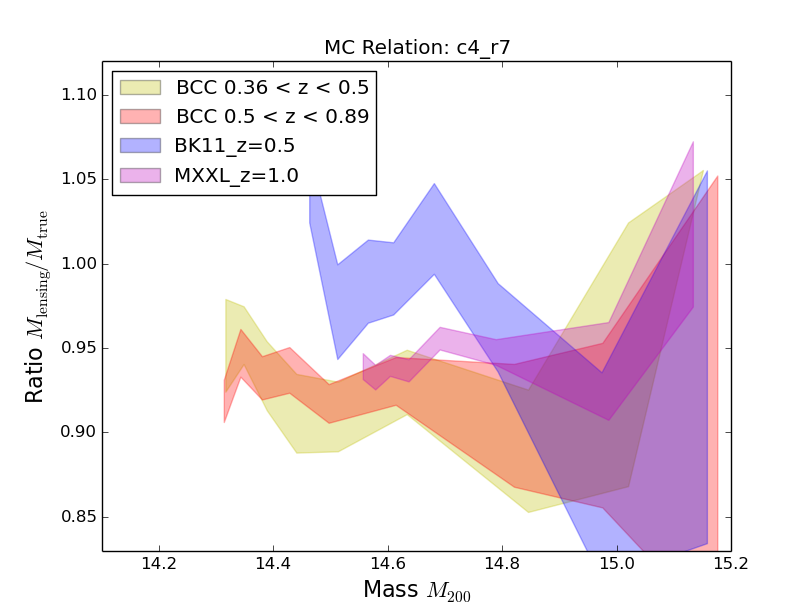
\includegraphics[width=0.3\textwidth]{figures/c4_r7}
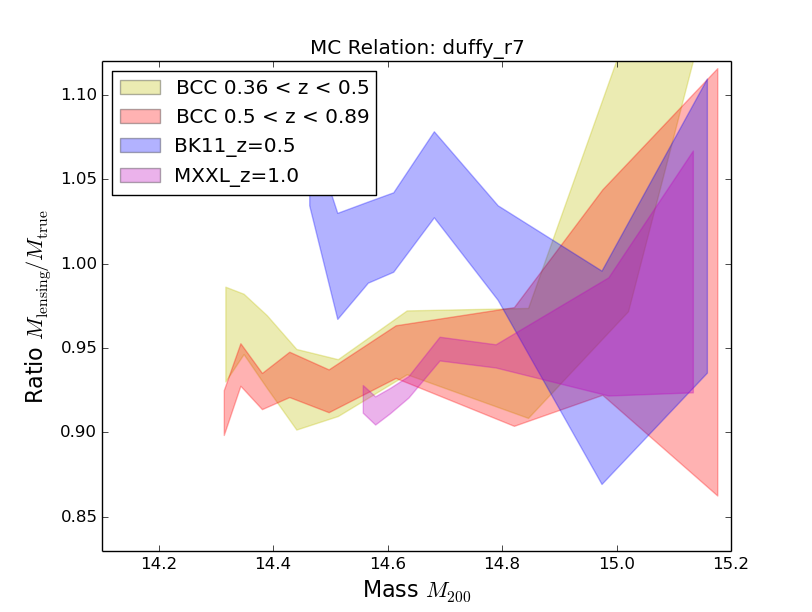
\includegraphics[width=0.3\textwidth]{figures/duffy_r7}
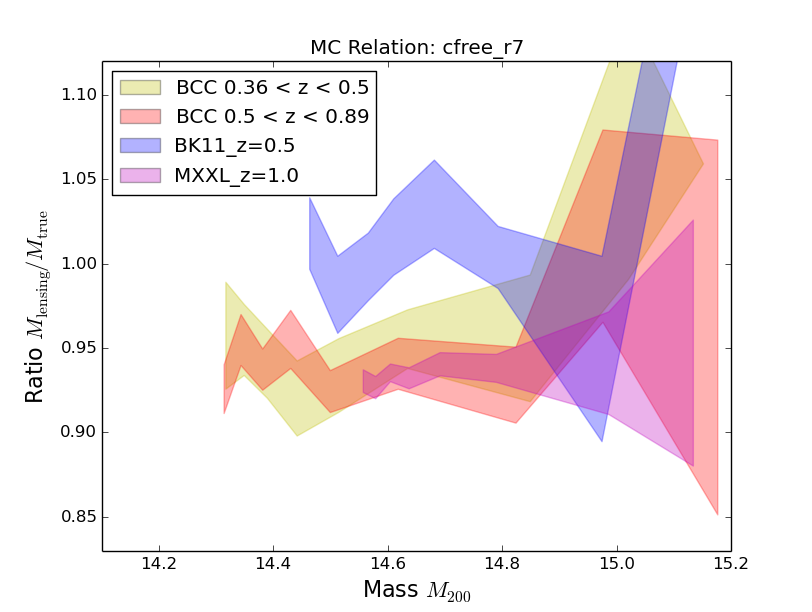
\includegraphics[width=0.3\textwidth]{figures/cfree_r7}
\caption{Plot of bias versus mass. Left: Assuming c=4, Center: Assuming Duffy08, and Right: C is a free parameter. The fit range is 0.5 - 3.0 Mpc. The width of each colored band represents the $1\sigma$ uncertainty in the median bias for each mass bin. Bins are adaptively created to balance signal-to-noise with exploring the mass range. Note from sec~\ref{sec:bcc_smothing}, I don't expect the BCC lines to be accurate here. Made with compareDiffSims.py}
\label{fig:comparing_r7_bias}
\end{figure}

The agreement between BCC and MXXL seems to be fit range dependent. The above fits covered a range of 0.5 - 3.0 Mpc. If we only look at the outer region for cfree, the fits are again good.

\logfig{figures/cfree_r10}{Same as fig~\ref{fig:comparing_r7_bias}, except now only for cfree and 0.75-3Mpc.}

However, if we look at the innermost fit region, 0.25-0.5 mpc, we can see that the two simulations are drastically different. BCC and BK11 show diving calibrations at the high mass end (0.2 for $10^{15}$ halos!?), but MXXL holds relatively steady up to the highest masses. 

\logfig{figures/cfree_r1}{Same as fig~\ref{fig:figures/cfree_r10}, except for on a radically different scale.}

This is apparently a resolution effect (see sec~\ref{sec:bcc_smoothing}. 


\subsection{Role of Mass-Concentration Relation}

I think that the behavior of the fits against the different mass-concentration relations vs cfree suggests that the simulations have intrinsically different m-c relations. This is supported by the work of \citet{ludlow_mc}, which shows that even for $M_{200} = 10^{14}$ clusters, the mean concentration can vary by 20\% over the WMAP1-7 and Planck cosmologies. 

This to me suggests a 2-pronged strategy. When we don't care about cosmology, for example, just talking about masses, then we can fix a mass-concentration relation (appropriate for that cosmology). However, for purposes of cosmological fits, we need to vary the m-c relation systematically over all clusters inline with the fit. That way we don't get hit by some ``systematic uncertainty'' by assuming an M-C relation, and we capture the covariance with cosmology.

%%%%%%%%%%%%%%%%%%%%%%%%%%%%%%%%%%%

\subsection{Testing a Cosmology-Dependent Mass-Concentration Relation}
\label{sec:cosmo_dependent_mc}

On Becker's suggestion, I tried out the Zhao08 model for cosmology dependent m-c relations, from \citet{zhao_cosmodepmc}, since they provide an online calculator and code. A calculator is at: \url{http://202.127.29.4/dhzhao/mandc.html}. In short, this more complicated M-C relation did not bring agreement as well as I had hoped.

\begin{figure} \centering
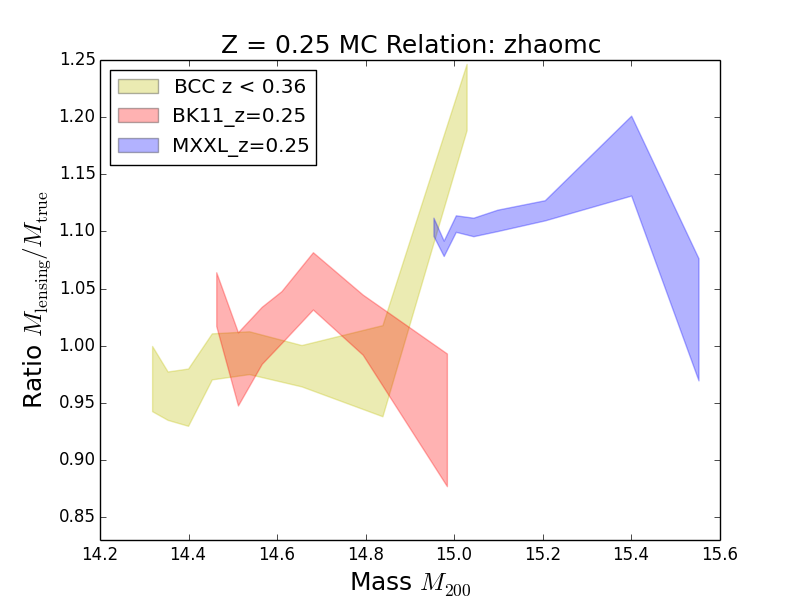
\includegraphics[width=0.4\textwidth]{figures/zhaomc_z25.png}
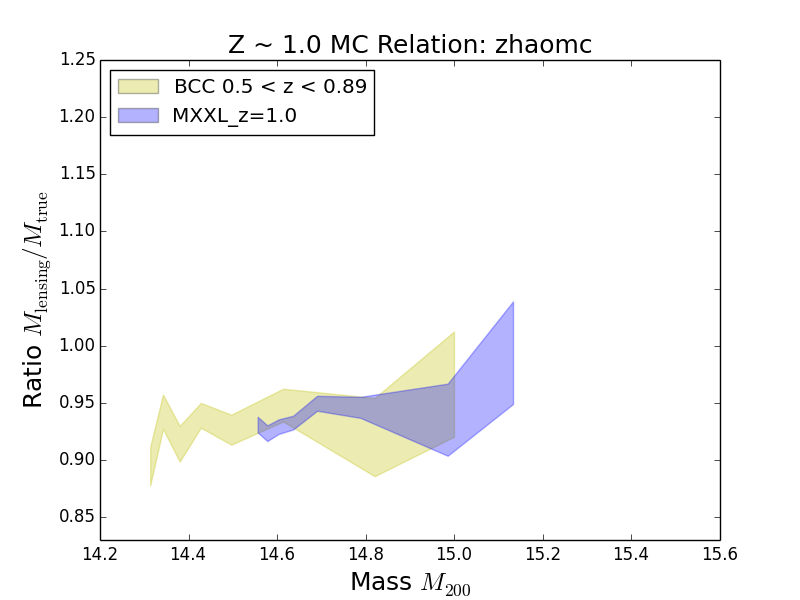
\includegraphics[width=0.4\textwidth]{figures/zhaomc_z10.png}
\caption{Median bias measured from the BCC, MXXL, and BK11 simulations using the Zhao M-C relation at left: $z=0.25$ and right: $z\approx 1.0$. Agreement is not disheartening, but is not signficiantly improved, either.}
\label{fig:zhamoc}

\end{figure}



%%%%%%%%%%%%%%%%%%%%%%%%%%%%%%%%%%


\subsection{Agreement Between Simulations with Free Concentration}
\label{sec:consistancy}

\begin{figure} \centering
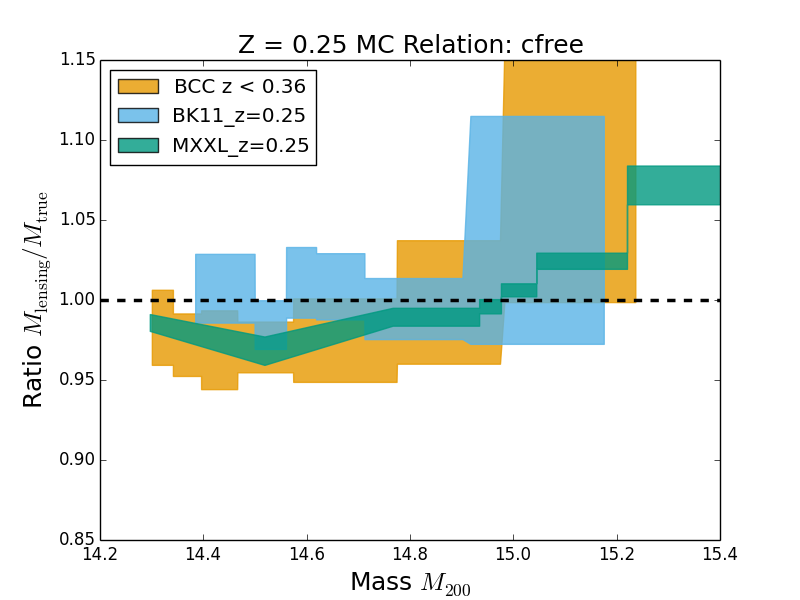
\includegraphics[width=0.6\textwidth]{figures/cfree_z25.png} \\
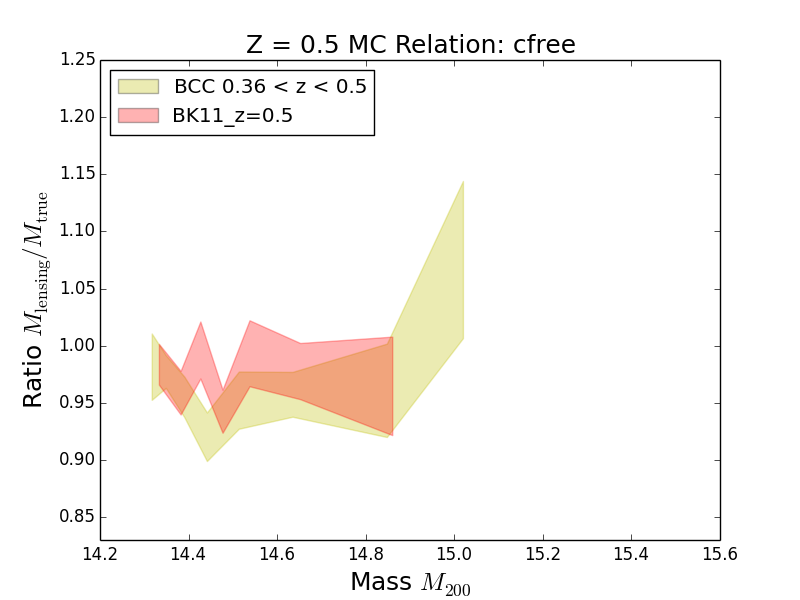
\includegraphics[width=0.6\textwidth]{figures/cfree_z5.png} \\
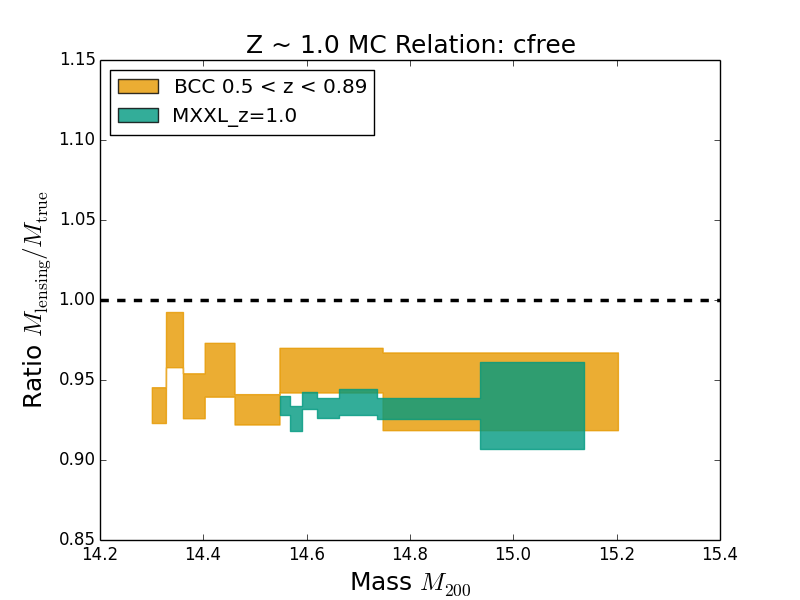
\includegraphics[width=0.6\textwidth]{figures/cfree_z10.png}
\caption{Median bias with concentration free, for fit range 750kpc - 3Mpc. Simulations seem to show good agreement.}
\end{figure}

So at least where we expect the simulations to agree, their median bias seems to agree. 
That's positive.
However, why is BK11 mildly higher than BCC and MXXL?


\begin{figure}\centering
  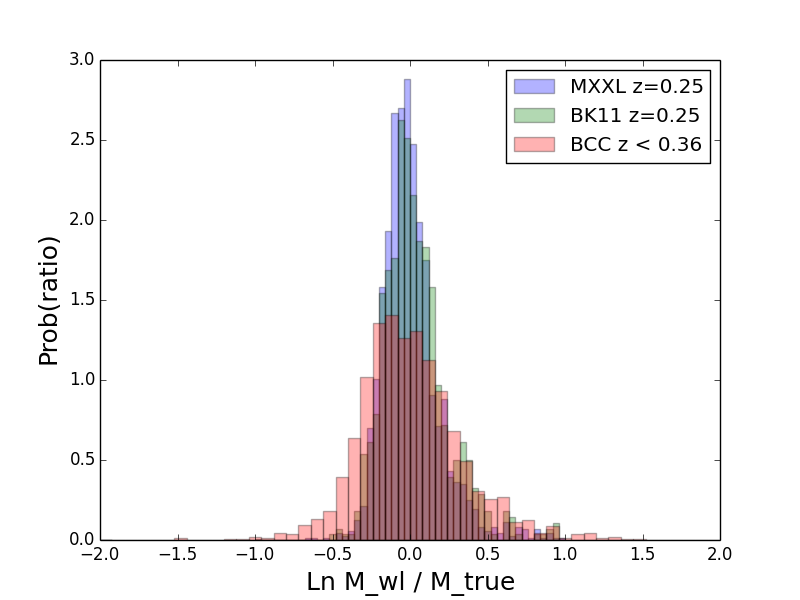
\includegraphics[width=0.4\textwidth]{figures/lowz_logscatter.png}
  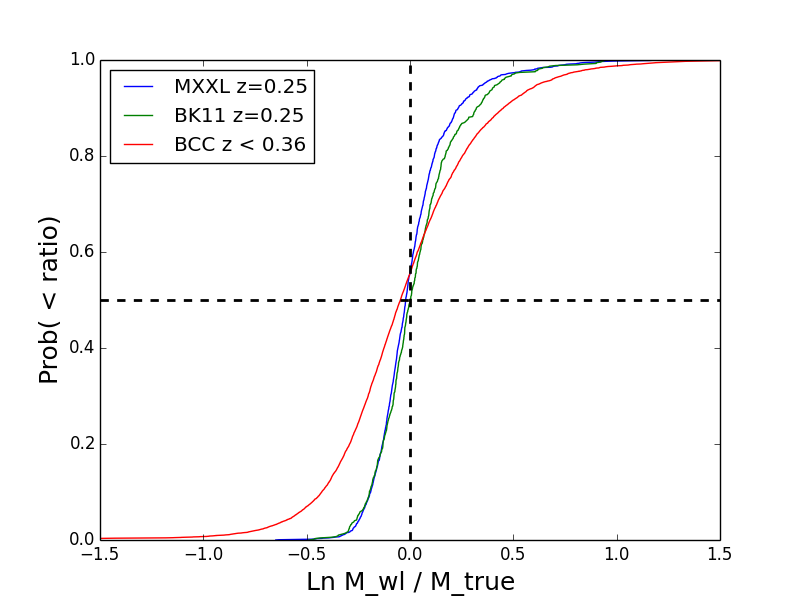
\includegraphics[width=0.4\textwidth]{figures/lowz_logscatter_cdf.png}
\caption{Scatter in recovered masses versus true masses. First, the scatter in the BCC is much larger since only that simulation measures the full LoS noise. Second, MXXL and BK11 seem to agree in their distribution at the low scatter, but the BK11 has slightly more up scatter. A KS test says that this is significant at $p=0.0024$, for $D=0.081$. However, maybe this is just the fact that BK11 has twice the LoS integration as MXXL? }
\end{figure}

This points towards a possibly scary conclusion. Can we not know the bias without folding in the full LoS scatter? But...the BCC settles back to the MXXL value! So maybe its not so bad anyway? Or is there something different about the LoS scatter in BK11?

Also, what causes the tail to high overestimates? This was seen and clearly measured by Matt in BK11. But he doesn't discuss a cause.


%%%%%%%%%%%%%%%%%%%%%%%%%%%%%%%%%%%%%


\subsection{Next Tasks}

\begin{itemize}
\item Inspect clusters that are in the highly skewed tail. Is there anything characteristic about their shear profiles?
\item Download and analysize BK11 simulations with only 200Mpc integration length. Is the scatter distribution consistant with the MXXL?
\item Can I recover the scatter in Bk11 and BCC by convolving the measured MXXL scatter with an appropriate function?
\end{itemize}




%%%%%%%%%%%%%%%%%%%%%%%%%%%%%%%%%%%%%%%%%%%%%%%%%%%%%%%%%%%%%%%%%%%%%%%%%%%%%%%%%%%%%%%%%%%%%%%%%%%%%%%%%%%%%%%%%%%%%%%%%%%%%%%%%%%%%%%%%%%%%%%%%%%%%%%%%%%%%%%%%%%%%%%%%%%%%%%%%%%%%%%%%%%%%%%%%%%%%%%%%%%%
%%%%%%%%%%%%%%%%%%%%%%%%%%%%%%%%%%%%%%%%%%%%%%%%%%%%%%%%%%%%%%%%%%%%%%%%%%%%%%%%%%%%%%%%%%%%%%%%%%%%%%%%%%%%%%%%%%%%%%%%%%%%%%%%%%%%%%%%%%%%%%%%%%%%%%%%%%%%%%%%%%%%%%%%%%%%%%%%%%%%%%%%%%%%%%%%%%%%%%%%%%%%
%%%%%%%%%%%%%%%%%%%%%%%%%%%%%%%%%%%%%%%%%%%%%%%%%%%%%%%%%%%%%%%%%%%%%%%%%%%%%%%%%%%%%%%%%%%%%%%%%%%%%%%%%%%%%%%%%%%%%%%%%%%%%%%%%%%%%%%%%%%%%%%%%%%%%%%%%%%%%%%%%%%%%%%%%%%%%%%%%%%%%%%%%%%%%%%%%%%%%%%%%%%%
\clearpage \newpage



\section{Optimal Radial Ranges for NFW Profiles}

Question: What is the best radial range to use when fitting an NFW profile? I need to provide answers in two different regiemes, which in the end may end up overlapping. The first is the SPT regime, where the limited field of view on Hubble restricts how far out we can probe. The second regime is ground-based wide-field data from Subaru or LSST, where we can go out as far as we want.

I ran 15 different fit ranges (see~\ref{sec:consistant_bias_mcrelation}) for all 3 simulations. Right now I am biased towards MXXL, so I will only show results for that at the moment.

\logfig{figures/cfree}{Plotting mass bias from lensing versus cluster mass, using the MXXL simulation and no m-c relation, for different radial ranges. Line styles denote different inner fit boundaries, while color denotes different outer fit boundaries. Color are grouped, suggesting that the outer fit boundary is more important than the inner fit boundary. Produced with compareSims.py}

Outer fit range seems to matter much more than inner fit range. You might expect that the behavior changes as the fit includes or excludes r200. R200 is at ~1.1Mpc for $10^{14.5}$ clusters, whereas it is closer to 1.4Mpc for $10^{15}$ clusters. So for example, fitting out to 1Mpc is inside R200 for all clusters, and that bias seems to stay pretty level for all masses (the last bin is noisy). The pink line, fitting to 1.5mpc, is somewhat outside R200 for the lighter clusters, and just barely outside for the most massive -- that line shows larger cluster masses at higher true masses. If for some reason fitting m\&c biases masses up, then the pink line could be converging to the ``right'' answer at higher masses. Similar story for 2.5 and 3 Mpc, where masses are notably underestimated at low masses, and the trend heads to less bias at higher masses. I'm not sure how to explain the green lines, fitting to only 750kpc. 


\textbf{Could I fit perfect NFW halos and add noise? That way I could see the effects of noise bias on a two parameter fit?}


\logfig{figures/cfree_scatter}{Plotting intrinsic scatter versus mass for different radial ranges, using the MXXL simulation and no m-c relation. Same coloring and line scheme as fig.~\ref{fig:figures/cfree}. Scatter increases as I limit the outer radius used in the fit.}

The story with the scatter is much clearer. As I move the outer radial range to small values, the amount of scatter picks up. As soon as I move inside R200, the scatter blows up. Why is this? Smaller area, so subject to more LSS noise? More substructure in clusters?

%%%%%%%%%%%%%%%%%%%%%%%%%%%%%%%%%%%%%%%%%%%%%%%%%%%%%

\subsection{Dealing with the Outer Fit Range}
\label{sec:outerfitrange}

Looking at figures \ref{fig:figures/cfree} and \ref{fig:figures/cfree_scatter}, the outer fit range seems to control the bias. And for each choice, there is a different mass dependence, probably described by how $R_{\mathrm{vir}}$ passes through the fit range for the masses I'm considering. It seems silly that the bias is this sensitive to the fit range, when in many cases the fit range isn't even something that I can control.

This bias comes from the fact that an NFW halo is a bad description of a cluster at distances beyond the virial radius. The NFW halo cuts off, and eventually a 2-halo term kicks in. Becker points this out in Fig 2 of his paper \citep{becker11}, and it goes along with other work by \citet{oguri_profiles} and \citet{tavio_profiles}, both of which propose suggested functional forms to model the density profile beyond the virial radius. Figure~4 in \citet{tavio_profiles} is particularly interesting, because he plots the rms scatter in the density profile as a function of radius. Above the virial radius, the rms scatter explodes from 20\% to 100\% by 2*$R_{\mathrm{vir}}$. Regardless of the functional form, this translates into a huge uncertainty in the shear profile of an individual cluster. So imagine if we included that theoretical uncertainty when fitting clusters? The fit would basically ignore any data above the virial radius, while self consistantly calculating the virial radius. That's exactly what the iterative method in \citet{becker11} tried to do, but without the iteration.

I've tried implimenting this in code. At r200, I started ramping up the uncertainty, and made the uncertainty really large outside r200. The result? The fitter removed all mass from the halo, so that all the measured signal was outside r200. That of course squashes chisquared. Messing around with masses versus r200 radii, I just don't think this will work. For any mass less than 1e14, r200 is barely inside 750kpc, especially at higher redshifts. I could make the prior tighter, but then I can't properly catch how the uncertainty tails to low mass.

%%%%%%%%%%%%%%%%%%%%%%%%%%%%%%%%%%%%%%%%%%%%%%%%%%%%%

\subsection{Next Steps}

For the HST proposal (due to STSCI in April, but need it for proposal writing by 25 Feb 2014), I need to add shape noise, use a lower sampling density, and apply HST masks associated with our mosaicing programs. That way I can directly measure the expected scatter for different choices, which will affect how powerful the HST program will be. 

There are some more general steps that I would like to do as well:
\begin{itemize}
\item Noise. I want to understand how the 2-parameter fit responds to noise. I could create perfect NFW halos and add shape noise to see how the best fit value changes. I also want to explore the 2D posterior surface for some of the clusters in MXXL, both relaxed and unrelaxed. Related, how does the posterior perform when I marginalize over it instead of using a point estimator?
\item We may in the end use a 1-parameter fit, but since the M-C relation is cosmology dependent, I need to implement a cosmology dependent relation. How does that perform?
\item Does the bias simplify if I add a ton of extra uncertainty at radii beyond the virial radius?
\end{itemize}



%%%%%%%%%%%%%%%%%%%%%%%%%%%%%%%%%%%%%%%%%%%%%%%%%%%%%%%%%%%%%%%%%%%%%%%%%%%%%%%%%%%%%%%%%%%%%%%%%%%%%%%%%%%%%%%%%%%%%%%%%%%%%%%%%%%%%%%%%%%%%%%%%%%%%%%%%%%%%%%%%%%%%%%%%%%%%%%%%%%%%%%%%%%%%%%%%%%%%%%%%%%%
%%%%%%%%%%%%%%%%%%%%%%%%%%%%%%%%%%%%%%%%%%%%%%%%%%%%%%%%%%%%%%%%%%%%%%%%%%%%%%%%%%%%%%%%%%%%%%%%%%%%%%%%%%%%%%%%%%%%%%%%%%%%%%%%%%%%%%%%%%%%%%%%%%%%%%%%%%%%%%%%%%%%%%%%%%%%%%%%%%%%%%%%%%%%%%%%%%%%%%%%%%%%
%%%%%%%%%%%%%%%%%%%%%%%%%%%%%%%%%%%%%%%%%%%%%%%%%%%%%%%%%%%%%%%%%%%%%%%%%%%%%%%%%%%%%%%%%%%%%%%%%%%%%%%%%%%%%%%%%%%%%%%%%%%%%%%%%%%%%%%%%%%%%%%%%%%%%%%%%%%%%%%%%%%%%%%%%%%%%%%%%%%%%%%%%%%%%%%%%%%%%%%%%%%%
\clearpage \newpage

\section{What are the effects of noise and sampling density on bias \& scatter?}
\label{sec:noisebias}

\subsection{Motivation}
I'm doing nonlinear fits to noisy data, and taking point estimates of the posterior. We generally expect that doing that will produce biased results. It may also explain the differences between BCC, MXXL and BK11 simulations. While all three simulations are noise-free, shear fields are sampled at different densities, which may have an effect.

\subsection{Set up}

I have submitted runs on the MXXL and BCC with different densities. All of the following are galaxies(samples) per square arcminute.
\begin{itemize}
\item 0: Default density
\item 1: 100 (MXXL only)
\item 2: 20 (MXXL only)
\item 3: 7
\item 4: 4  (MXXL only)
\item 5: 1  (MXXL only)
\item 6: 10
\end{itemize}
(19 Jan 2015 Note: The numbering was off. I was using much lower densities than I thought in many of the following tests).

I have used four different noise levels.
\begin{itemize}
\item 0: No noise
\item 1: 0.16 shape noise on tangential shear
\item 2: 0.33
\item 3: 0.5
\item 4: 0.4
\end{itemize}

I ran with c4 and cfree MC relations using the standard nfwfit.py software. Comparisons were made using the script compareSampling.py, and with the logfile compareSampling.log.


%%%%%%%%

\subsection{Does MXXL and BCC agree when using the same sampling density?}

We already know that the two simulations don't agree if c=4, so I will skip that.


\begin{figure} \centering
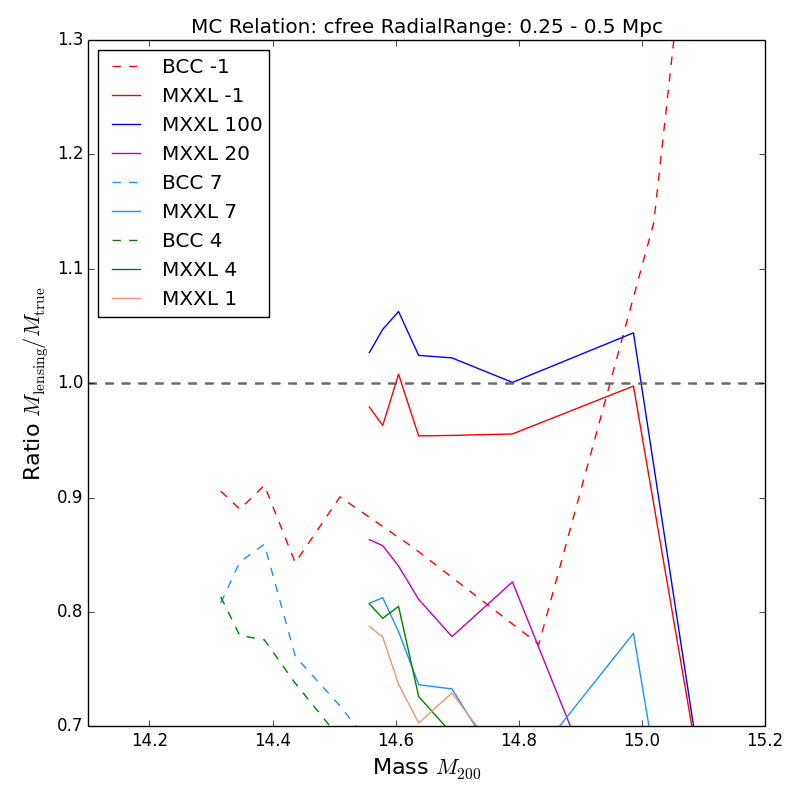
\includegraphics[width=0.3\textwidth]{figures/density_cfree-r1}
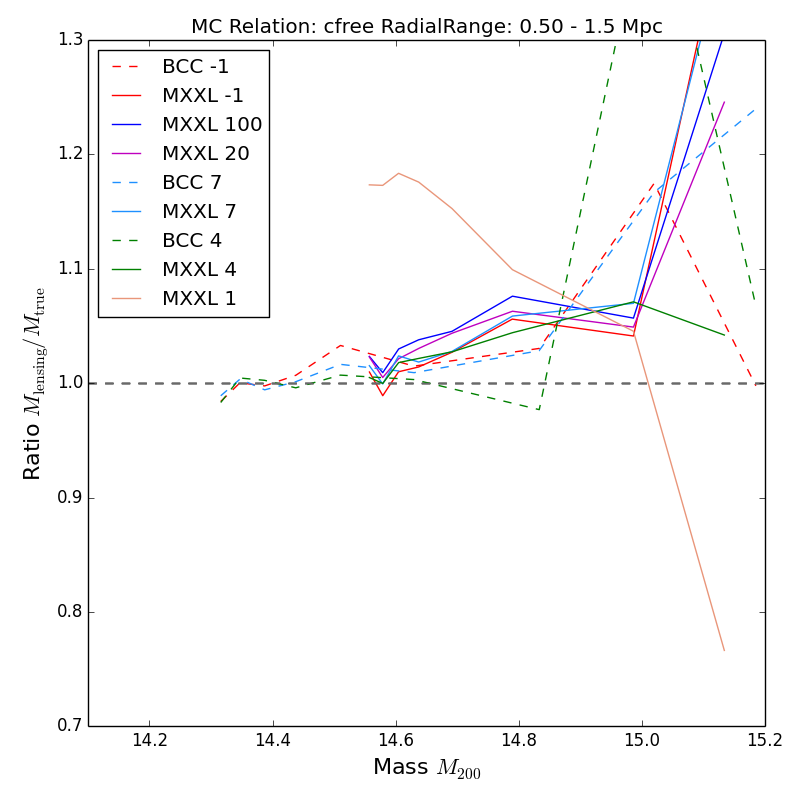
\includegraphics[width=0.3\textwidth]{figures/density_cfree-r5}
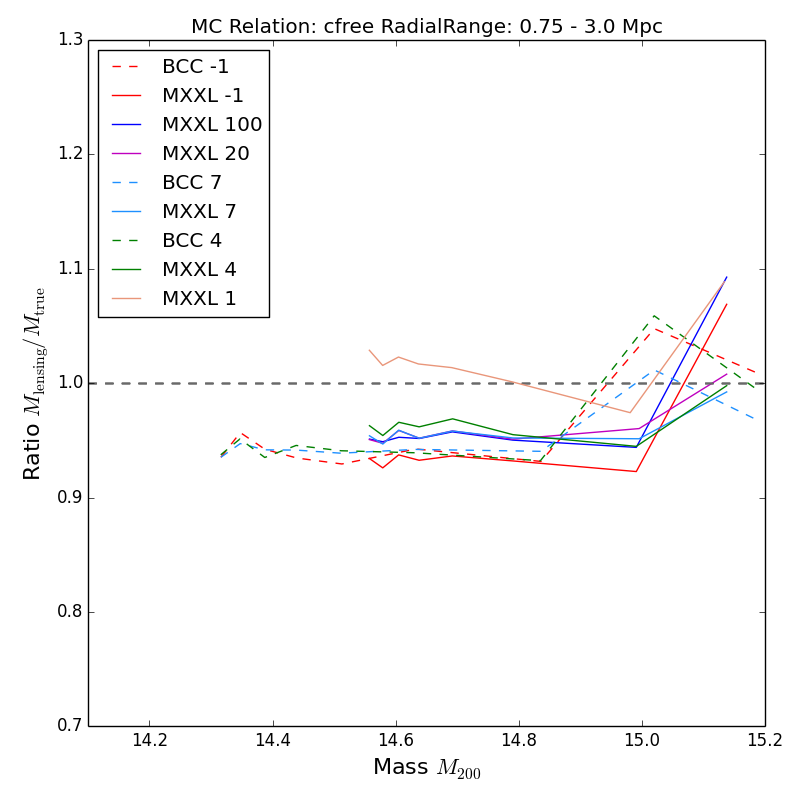
\includegraphics[width=0.3\textwidth]{figures/density_cfree-r10}
\caption{Bias measured from the BCC and MXXL simulations. No shape noise is added, but different sampling densities are used. Left, center, and right are using three different fit radii.}
\label{fig:bcc_vs_mxxl_density}
\end{figure}

We can see the bias comparison in figure~\ref{fig:bcc_vs_mxxl_density}. The center and right panels, fitting and 0.5Mpc and above, show a clean story. I would argue that the simulations roughly agree in the mass range where they have overlapping statistics. The correspondance breaks down a bit in the center panel, but again, rough agreement. In the left panel, we can see that density is really important. With enough sample points, the bias is well behaved (solid red and green curves). But sample sparsely, and the bias jumps up. But the two simulations roughly agree.

\begin{figure} \centering
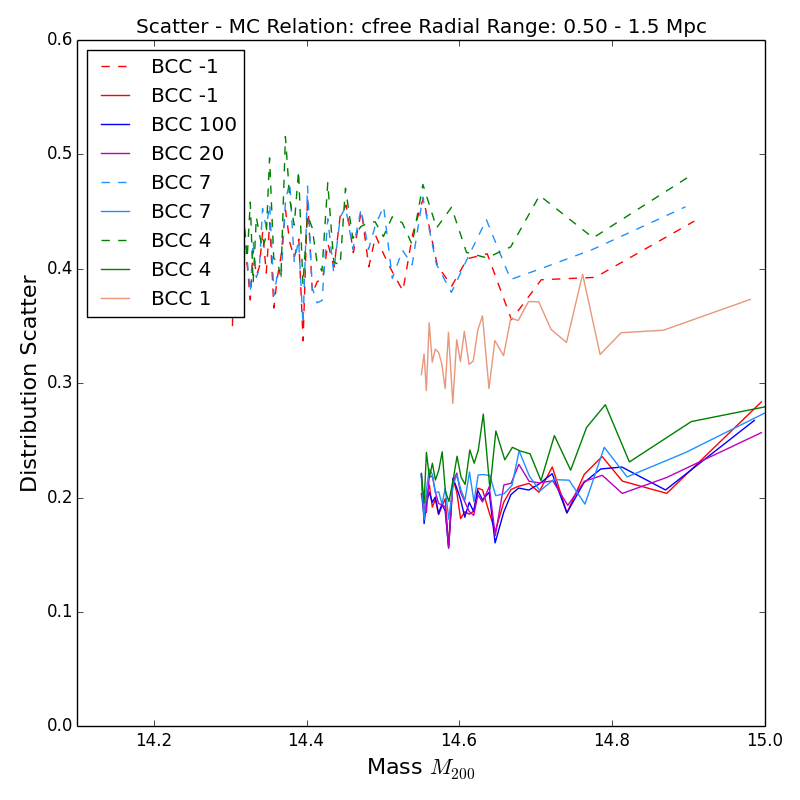
\includegraphics[width=0.4\textwidth]{figures/density_cfree-r5_scatter}
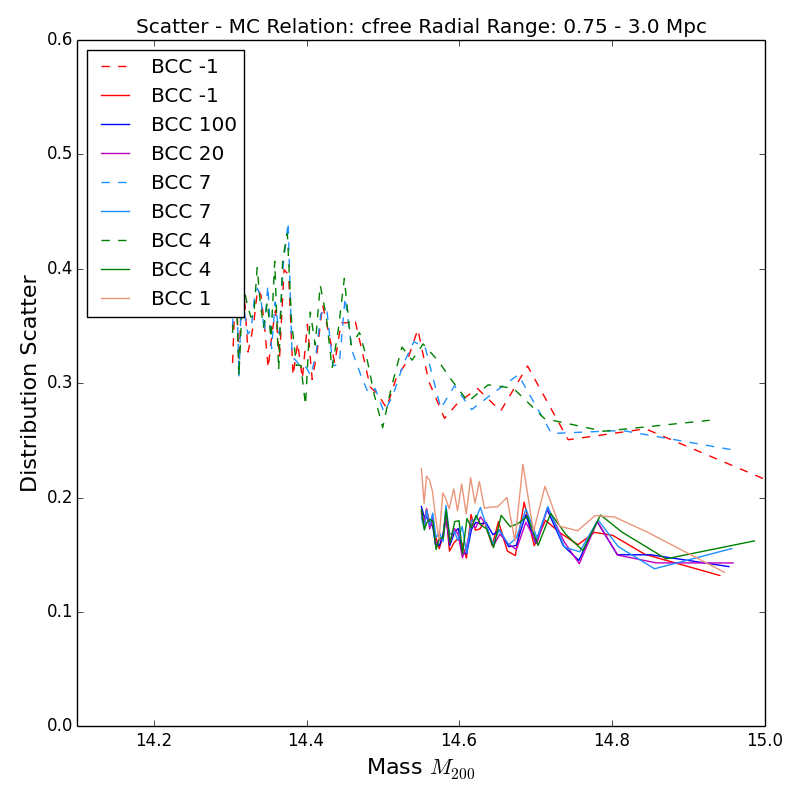
\includegraphics[width=0.4\textwidth]{figures/density_cfree-r10_scatter}
\caption{Comparison of recovered scatters from the two simulations.}
\label{fig:bcc_vs_mxxl_density_scatter}
\end{figure}

When it comes to the scatter, however, the two simulations do not agree. From figure~\ref{fig:bcc_vs_mxxl_density_scatter}, we see that the MXXL has a scatter of ~20\%, practically independent of sampling density. The BCC has a scatter of 30-40\%, with signs of mass dependence. Again, density does not appear to matter. 

\textbf{Why does the scatter not change as the sampling density is reduced (until very low density)?}
10x more noise, when the noise is non-existant, is still non-existant noise, no?

\subsubsection{Redshift evolution in BCC bias}

I broke down the BCC bias and scatter as a function of mass and redshiftin figure~\ref{fig:bcc_bias_redshift_evo}. This is only for the outer region. However, we see that there does appear to be evolution in the bias and scatter with redshift \emph{and} mass. However, the evolution in bias is < 10\%. I do not think that is enough to explain the extra scatter.

\begin{figure} \centering
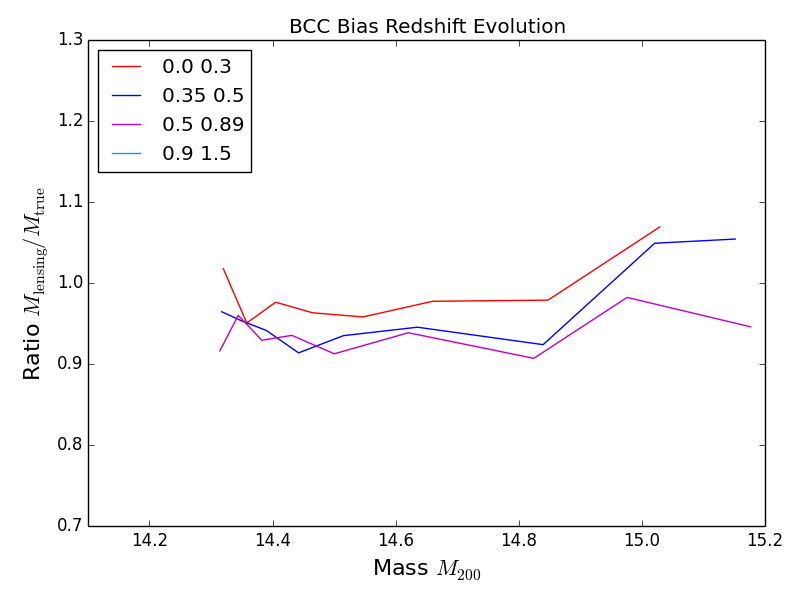
\includegraphics[width=0.8\textwidth]{figures/bcc_bias_redshift_evo_r10_n0_0}
\caption{Evolution of BCC calibration as a function of mass and redshift (colored lines). Left: Bias, Right: Scatter. We do see some redshift evolution(!). It does not appear to be enough to explain the extra scatter in the BCC, but it is important include when trying to calculate the actual bias expected.}
\label{fig:bcc_bias_redshift_evo}
\end{figure}

\subsubsection{Explaining BCC vs MXXL scatter differences with integration length}

Turns out Becker already thought about this in \citet{becker11}. MXXL only includes structure out to 200 Mpc $h^{-1}$, as did BK11. That captures all of the correlated scatter, and some but not all of the uncorrelated scatter. Becker used the calculation from \citet{hoekstra2003} to estimate how much extra noise comes from the rest of the LOS structure. For the lower-mass clusters in BK11 (Section 4.1 and Table 1), the extra LoS noise brings the scatter from $\approx22\%$ to $30\%$. The effect is much smaller for halos $M_{500} > 5\times10^{14}$, where only a few to 5\% points are added to the scatter.



\subsubsection{Sensitivity to Profile Assumptions}

The bias response from assuming an incorrect mass-concentration relation is cosmology dependent \emph{and} radial dependent. In figure~\ref{fig:profile_sensitivity_range_cosmo}, the bias as a function of mass changes with both variables in a way much larger than the difference between different sampling levels.

\begin{figure} \centering
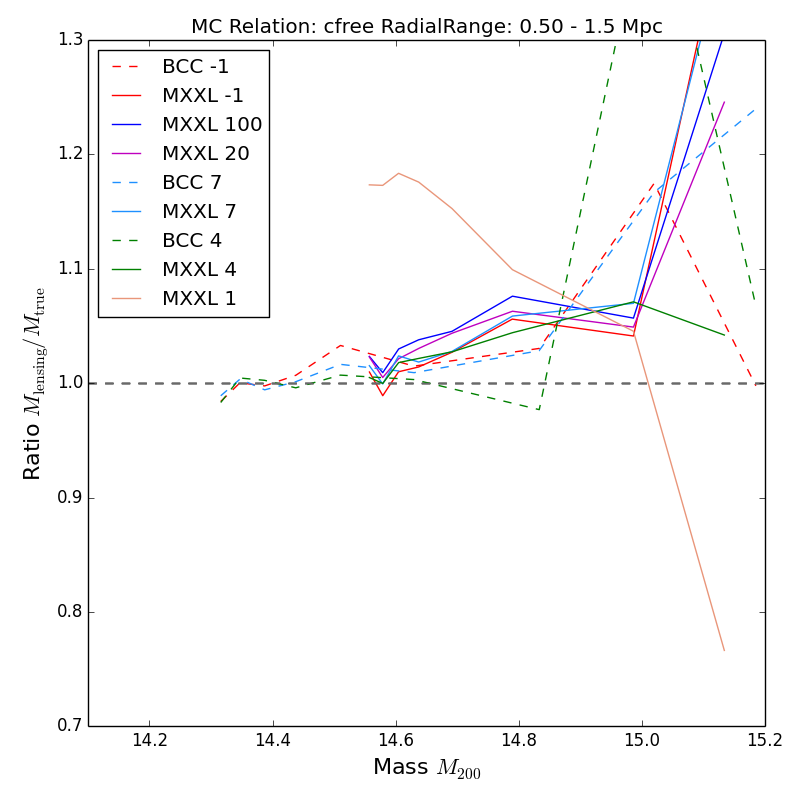
\includegraphics[width=0.4\textwidth]{figures/density_cfree-r5}
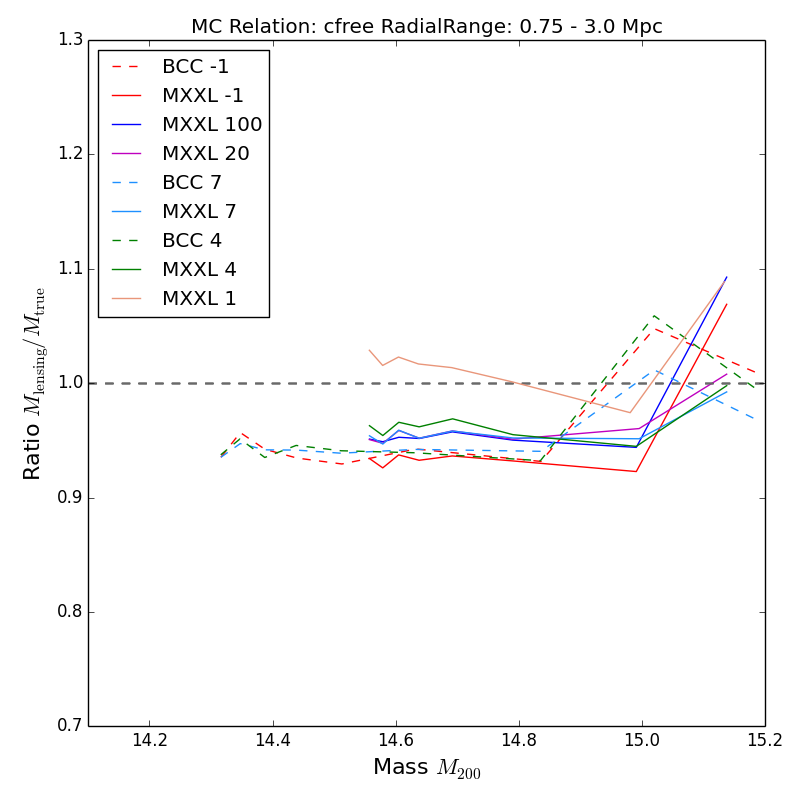
\includegraphics[width=0.4\textwidth]{figures/density_cfree-r10}\\
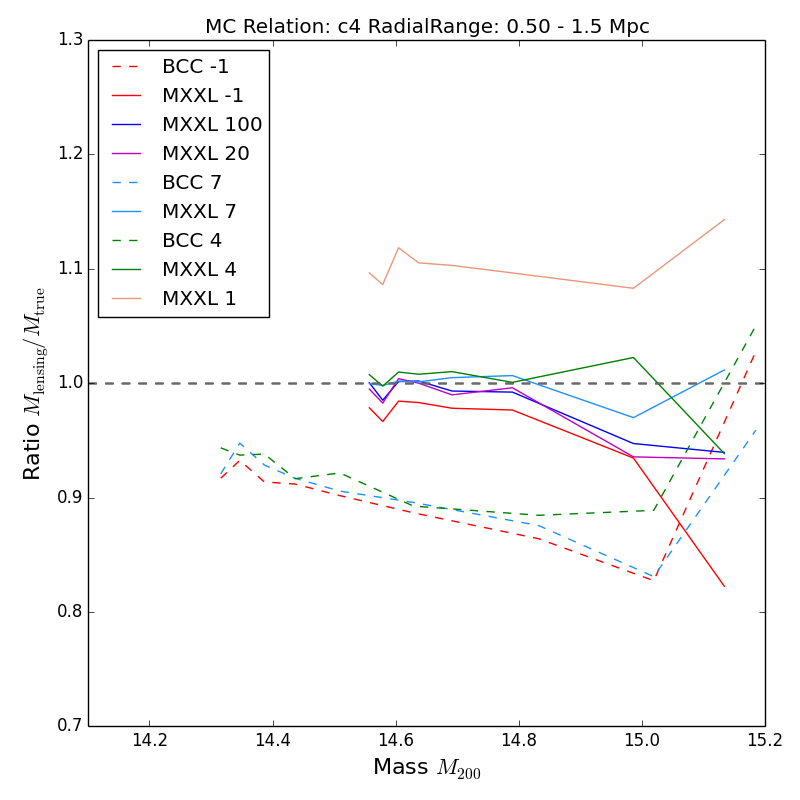
\includegraphics[width=0.4\textwidth]{figures/density_c4-r5}
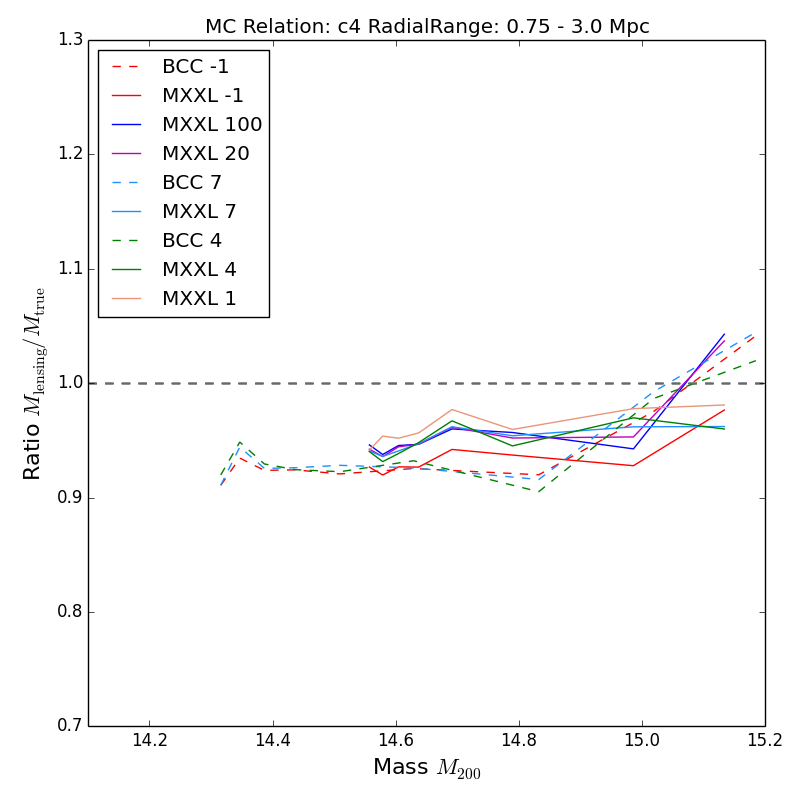
\includegraphics[width=0.4\textwidth]{figures/density_c4-r10}
\caption{A comparison of how the mass-dependent bias changes with cosmology, radial range, mass-concentration relation, and sampling density. Notice how freeing the concentration radically changes the bias, even for high noise simulations.}
\label{fig:profile_sensitivity_range_cosmo}
\end{figure}

%%%%%%%%%%%%%%%%%%%%%%%%%%%%%%%%%%%%%%%%%%

\subsection{To Consider: If bias depends on cosmology}

I've seen that the two simulations seem to agree when I fit for concentration, at large radii, but that breaks down some at the inner most radii. What if that difference is real, and caused by substructure? What if different cosmologies produce clusters with different amounts of substructure, which lead to different measured biases? 

First, we need to make sure the analysis is robust against substructure and m-c relation. But at some level, \emph{the expected bias has to be cosmology dependent!}

%%%%%%%%%%%%%%%%%%%%%%%%%%%%%%%%%%%%%%%%

\subsection{How does the posterior change as noise is added?}
\label{sec:noisebias_posteriors}

On Monday, I examined how the bias and scatter change as the noise levels change in the simulation. I noticed that the bias tends to increase with increasing noise. I think that is the effect of ``noise bias'', as in the posterior is becoming more skewed at high noise levels. I should be able to see that for individual halos. 

code: inspectProfiles.py
Logfile: logs/noisebias\_probsurface.log

Yeah, this is not working out so well. I think I'll need to table this until later.

%%%%%%%%%%%%%%%%%%%%%%%%%%%%%%%%%%%%%%%

\subsection{How does the bias \& scatter change as noise is added?}
\label{sec:noisebias_bias}

%%%%

\subsubsection{Scatter at high densities}

I'll start with 100 galaxies per sq arcminute. At the outer radii, this is a lot of samples even for noisy galaxies. The behavior of the scatter, however, has some odd radial dependence. See figure~\ref{fig:noisebias_highdensity_radrange}. The smaller fit range has noise that goes up uniformly. That to me suggests the noise is dominated by shape noise. At the outer radii, there are more galaxies included in the fit, so I guess shape noise is suppressed more. OK, not surprising then that the noise rises slower. However, the scatter develops a mass dependence. From the no noise case, we can see that the intrinsic LSS \& triaxial noise is not mass dependent. So maybe this is a signal strength effect, which gets swamped in the shape-noise dominated case at lower radii?

Note that fitting for concentration increases noise, but not radically, except at low radii.

\begin{figure}
\centering
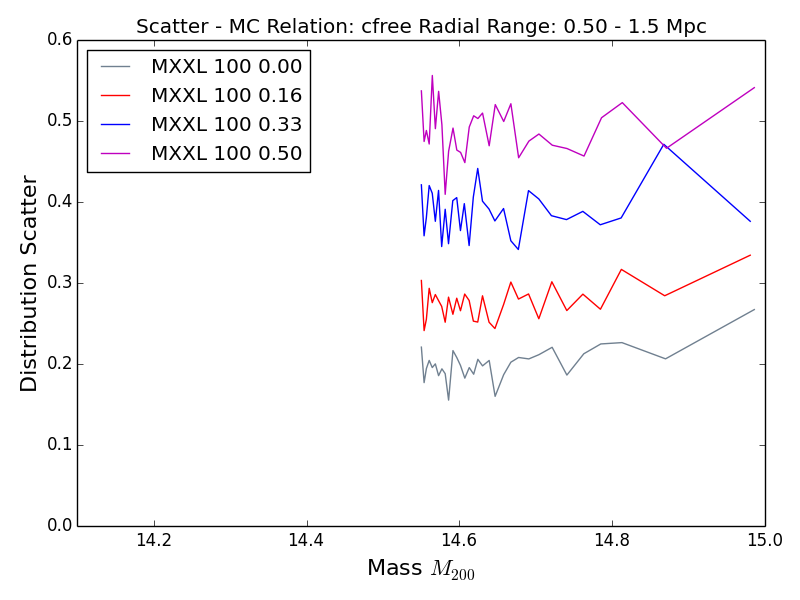
\includegraphics[width=0.4\textwidth]{figures/noise_cfree-r5-n1_3_scatter}
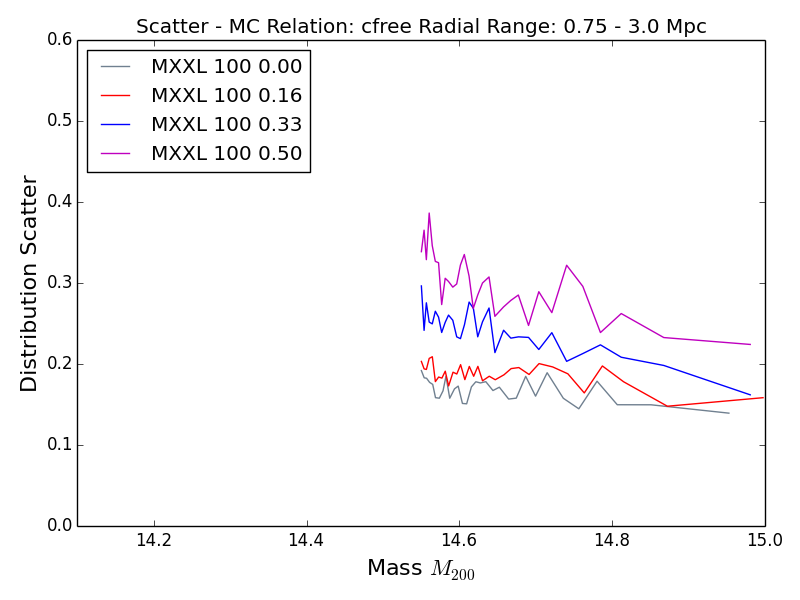
\includegraphics[width=0.4\textwidth]{figures/noise_cfree-r10-n1_3_scatter}\\
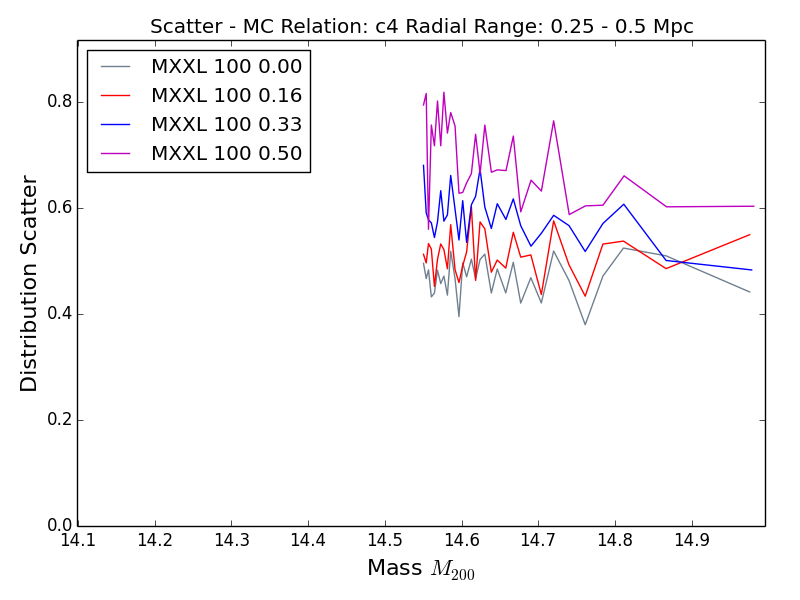
\includegraphics[width=0.4\textwidth]{figures/noise_c4-r5-n1_3_scatter}
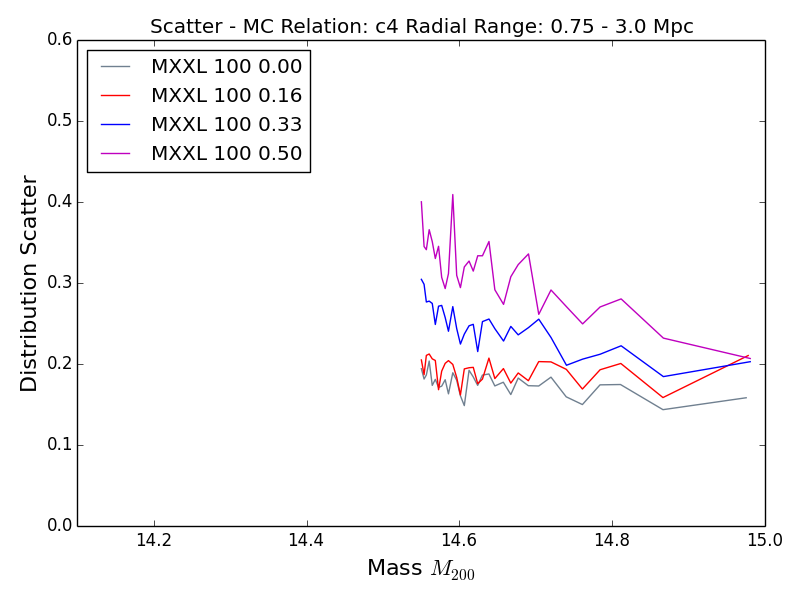
\includegraphics[width=0.4\textwidth]{figures/noise_c4-r10-n1_3_scatter}
\caption{Shown are the measured scatters for 100 galaxies per sq arcminute at different levels of noise. Left column shows fits to 0.5-1.5mpc, whereas the right column shows 0.75 - 3mpc. Top row has concentration free in the fits, the bottom row restricts c=4. Fits to 0.5-1.5mpc behave as I would expect: add shape noise, and the measured scatter goes up. However, fits to 0.75-3mpc show a mass dependence to the noise. While noise goes up, it goes up faster for the low mass galaxies, and at a rate slower than the smaller fit range.}
\label{fig:noisebias_highdensity_radrange}
\end{figure}

%%%%%

\subsubsection{Bias at high densities}

As was seen in \citet{bahe12}, added noise shifts the average bias up. However, at least at 100 galaxies per sq arcmin, the effect is not large, and is somewhat muddled. Also confusing is why the c-free fits to 0.5 - 1.5 mpc develops a mass-dependent bias. See Figure~\ref{fig:noisebias_highdensity_bias}.

\begin{figure}
\centering
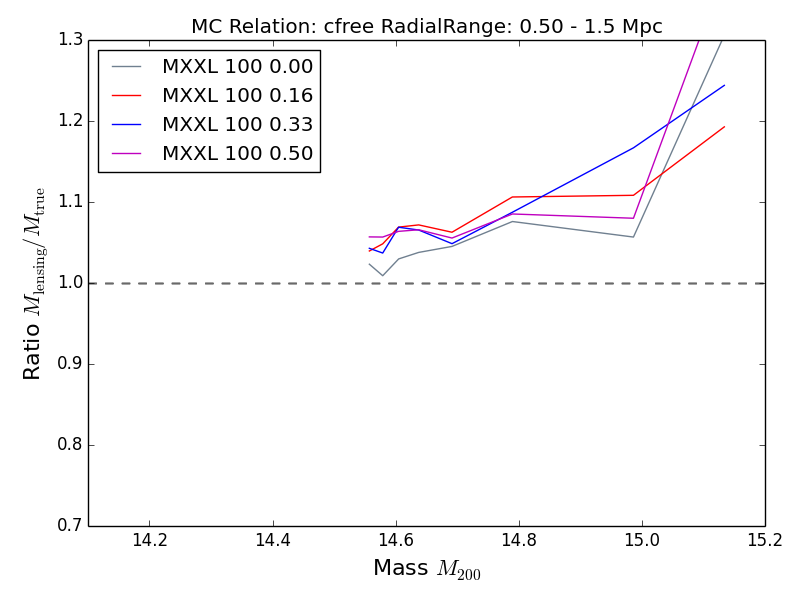
\includegraphics[width=0.4\textwidth]{figures/noise_cfree-r5-n1_3}
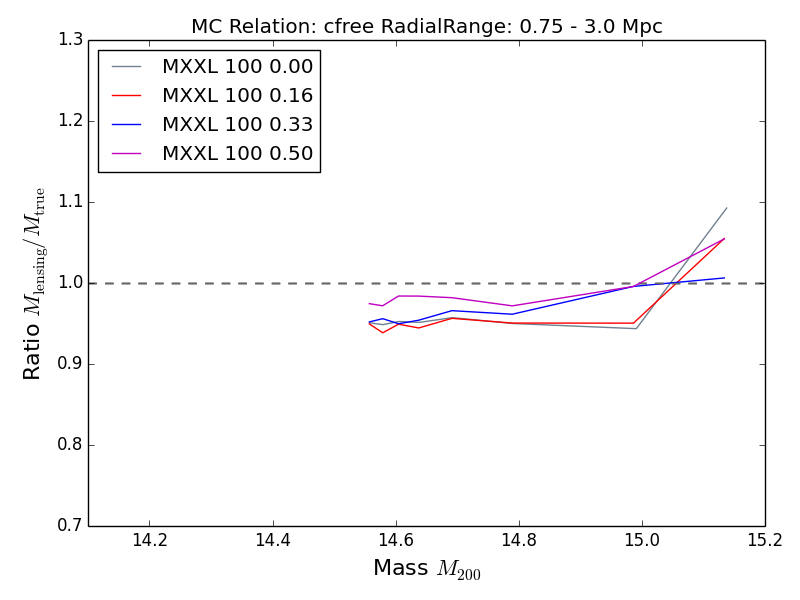
\includegraphics[width=0.4\textwidth]{figures/noise_cfree-r10-n1_3}\\
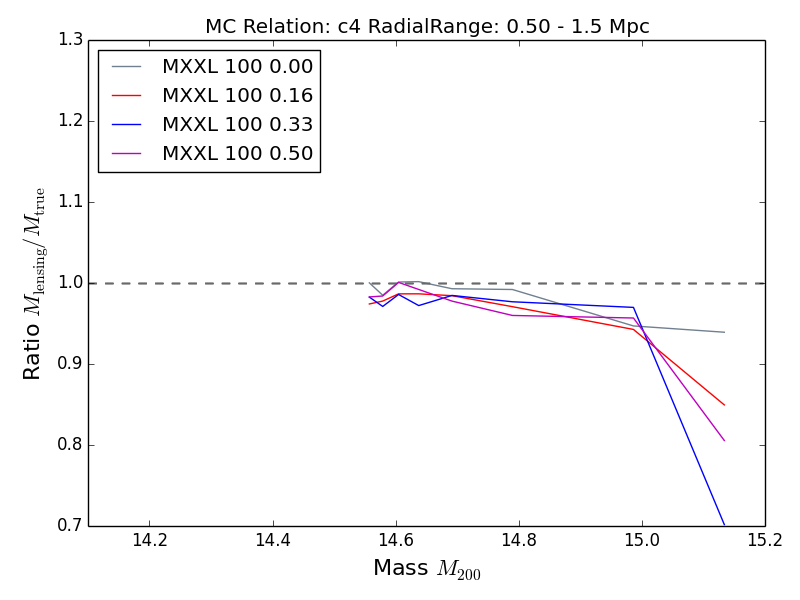
\includegraphics[width=0.4\textwidth]{figures/noise_c4-r5-n1_3}
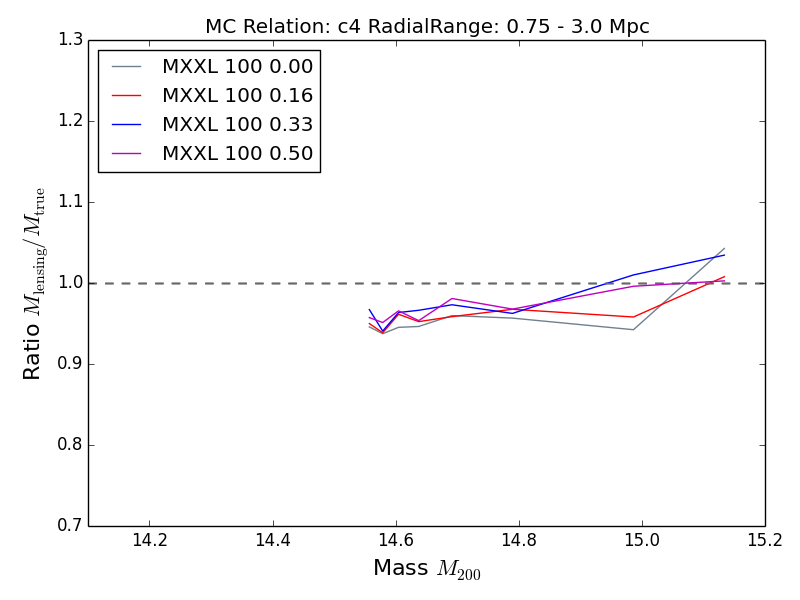
\includegraphics[width=0.4\textwidth]{figures/noise_c4-r10-n1_3}
\caption{Same as fig~\ref{fig:noisebias_highdensity_radrange}, except now I show the bias. What is odd is the c-free fit to 0.5-1.5 mpc, and there is a mass-dependent bias. This was seen previously in multiple figures earlier in this section.}
\label{fig:noisebias_highdensity_bias}
\end{figure}

%%%%%%%

\subsubsection{Bias vs sampling for noisy galaxies}

For the most dramatic example of how noise affects the bias, I turn to noisy galaxies, and change the sampling density at 0.75-3mpc. See figure~\ref{fig:noisebias_noisygals_sparsesampling}.

\begin{figure}
\centering
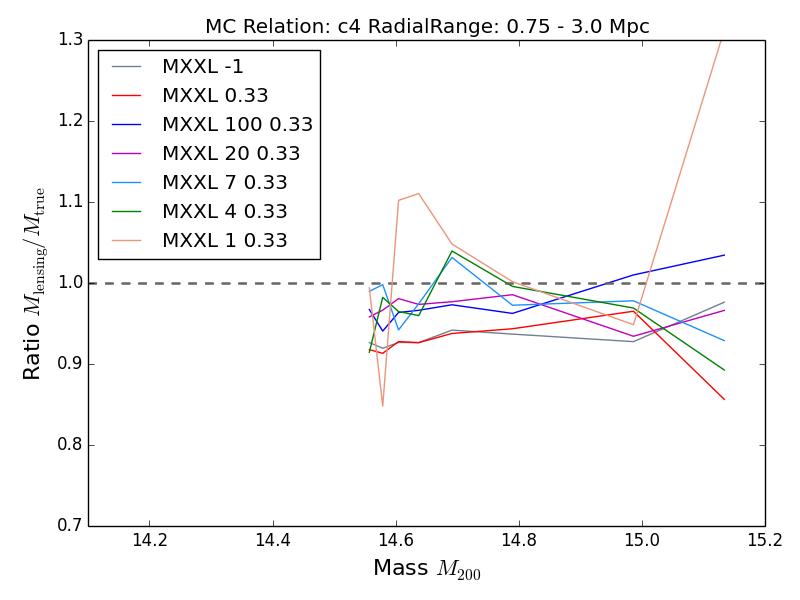
\includegraphics[width=0.4\textwidth]{figures/density_noise2_c4-r10}
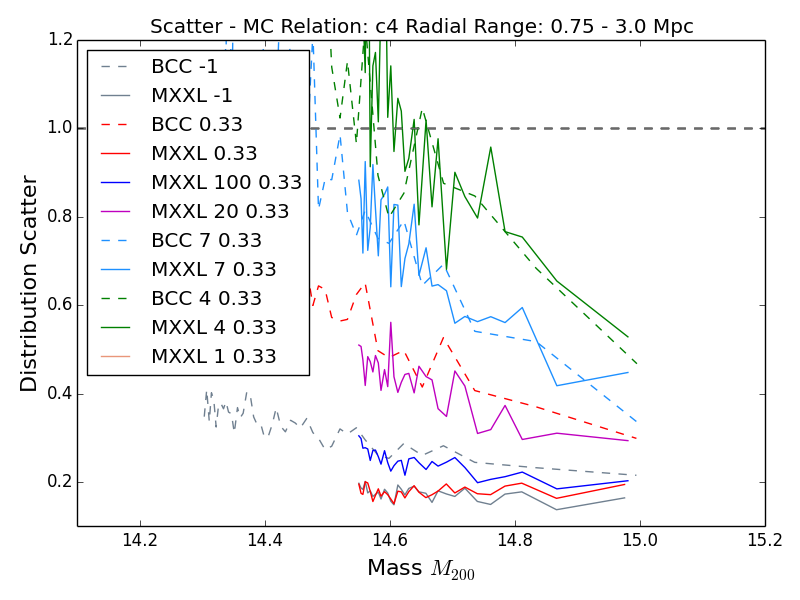
\includegraphics[width=0.4\textwidth]{figures/density_noise2_c4-r10_scatter}\\
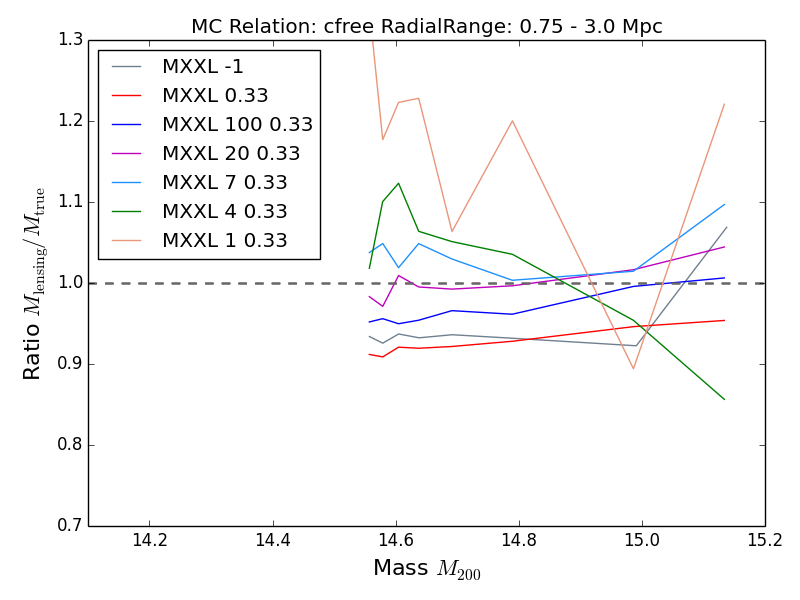
\includegraphics[width=0.4\textwidth]{figures/density_noise2_cfree-r10}
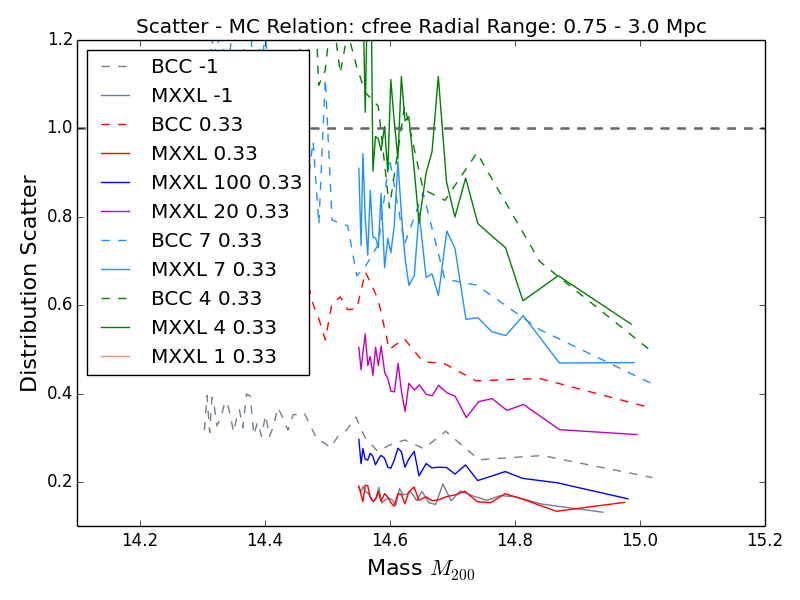
\includegraphics[width=0.4\textwidth]{figures/density_noise2_cfree-r10_scatter}
\caption{Plotted are simulations with increasing noise levels (fit at 0.75-3mpc). Top has c=4, bottom has c-free. The bias is similar at low noise, and seems to shift in similar ways, though the c=4 fit never shifts bias as much as c-free. Interestingly enough, the scatter does not increase dramatically at this radii when concentration is let free. This is in contrast to smaller radii. Obviously fitting for the concentration has an effect, as it changes the bias, but somehow it doesn't change the scatter.}
\label{fig:noisebias_noisygals_sparsesampling}
\end{figure}

Why does bias seems to increase in a mass independent way up to some noise point, after which lower mass clusters develop a steeper bias? The effects aren't as strong with c=4. But I suspect noise bias is at play here. The direction of the bias would suggest skewed posteriors, with tails to to low mass, and high probability density just above the correct mass. I will have to find a way to see that.

%%%%%%%%%%%%%%%%%%%%%%%%%%%%%%%%%%%%%%%%%%%%%%%%%%%%%%%%%%%%%%
%%%%%%%%%%%%%%%%%%%%%%%%%%%%

\subsection{Effects of Binning on Bias \& Scatter}
\label{sec:binningmethod}

When I fit to the innermost region, for example 0.25 Mpc - 0.5Mpc, we see some funky effects going on. Fig~\ref{fig:figures/cfree_r1} shows that MXXL and BCC disagree on the bias, and that BCC is a terribly negative bias in this inner fit range while MXXL does not. When we control for sampling density in Fig~\ref{fig:bcc_vs_mxxl_density}, we see that the MXXL bias moves to match the BCC bias. Could this simply be an artifact of how I bin the profiles? Currently I create radial bins with equal numbers of galaxies. At lower sampling densities, the inner most bin will stretch over a wider and wider radial range. Let us test that.

Using the MXXL, I ran every combination of:

\begin{itemize}
\item MC Relation: c4, cfree
\item Density: Full density, 7 galaxies/arcmin.
\item Radial Range: r11 (0.25 - 0.75), r5 (0.5 - 1.5), r6 (0.5 - 2.5), r10 (0.75 - 3)
\item Binning: Equal50, Equal200, Log6, Log12, Log18, Linear6, Linear12, Linear18
\end{itemize}


First, looking at large radial fits for fixed mass-concentration. Binning method appears to make a difference, however, the change in bias is roughly about 1 percentage-point. That's about half the difference of going from effectively infinite signal to 7 galaxies/arcmin. See fig~\ref{fig:density_binning_bias}. The story seems to be roughly the same for fits to 0.25 - 0.75, at for fits starting at 0.5 Mpc.

Once we let the concentration free, things get slightly more interesting. The fits to 0.75 - 0.3 Mpc still seem to be well behaved, and in fact have a very similar bias to the c=4 fits. Basically, those fits are insensitive to the m-c relation. Fitting with cfree to 0.25 - 0.75 is different. With high source density the bias shifts, but is relatively insensitive to binning (6\% point spread). Once the source density drops to something reasonable, then different profiles just go nuts to different biases. Equal binning sinks to very negative biases, linear and log binning appears to have a positive bias. Can't quite make out a pattern in terms of number of bins.

\begin{figure}
\centering
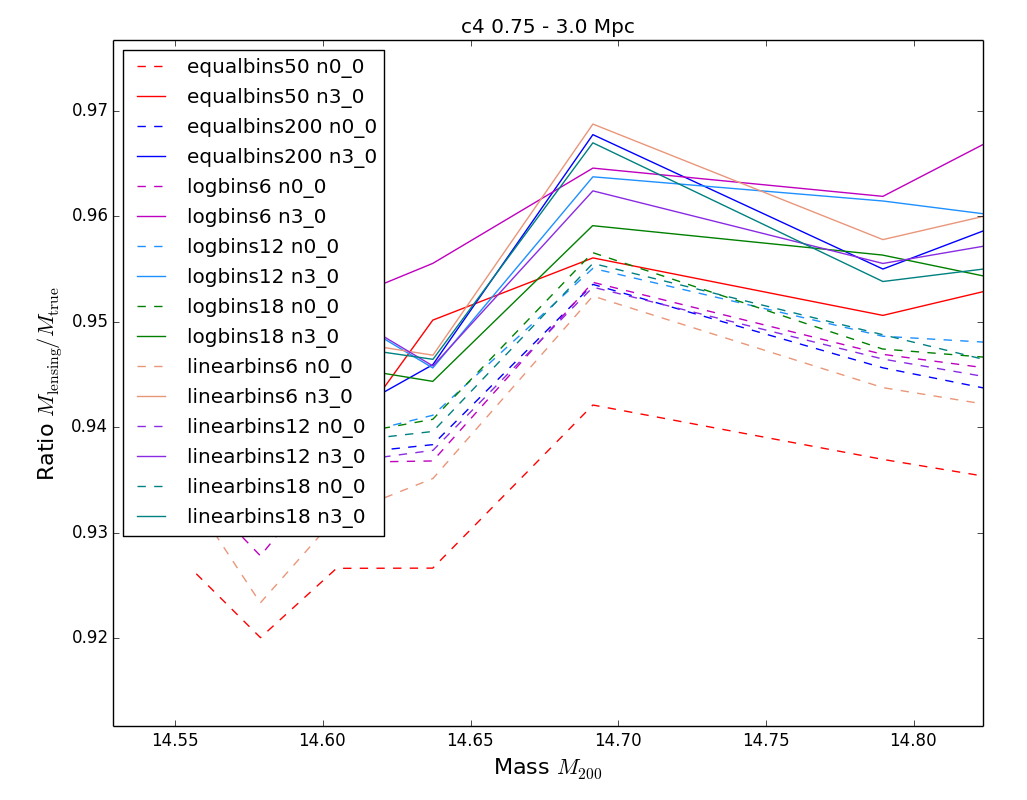
\includegraphics[width=0.45\textwidth]{figures/density_binning_wtg}
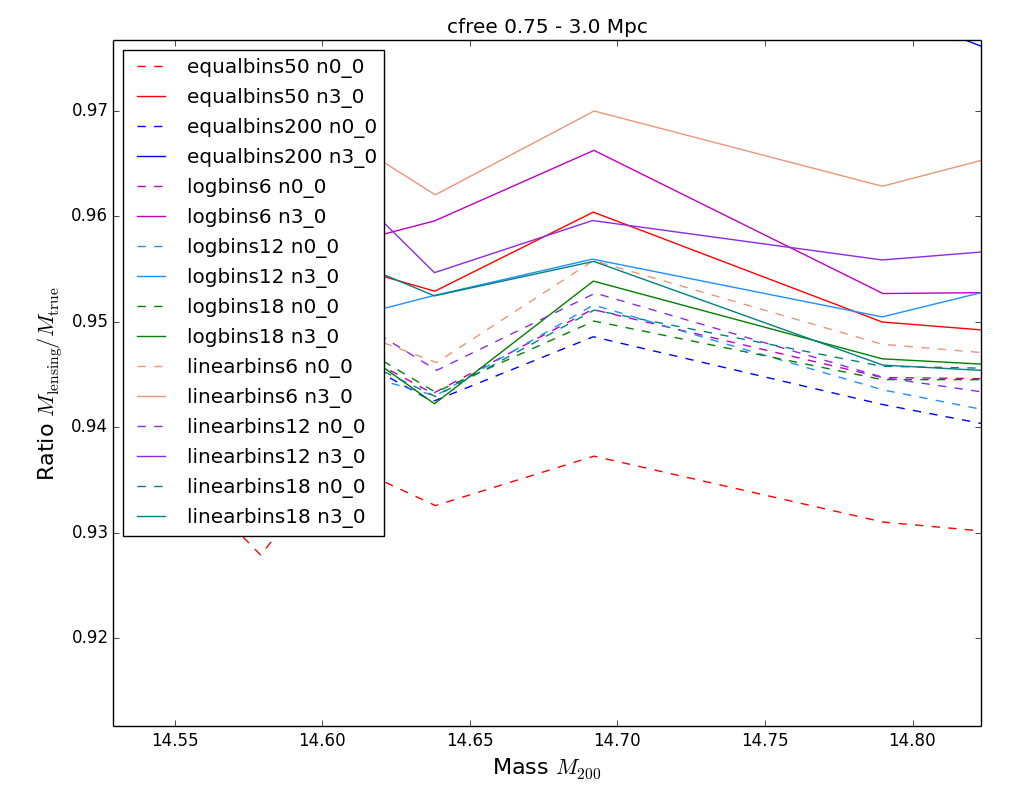
\includegraphics[width=0.45\textwidth]{figures/density_binning_wtg_cfree} \\
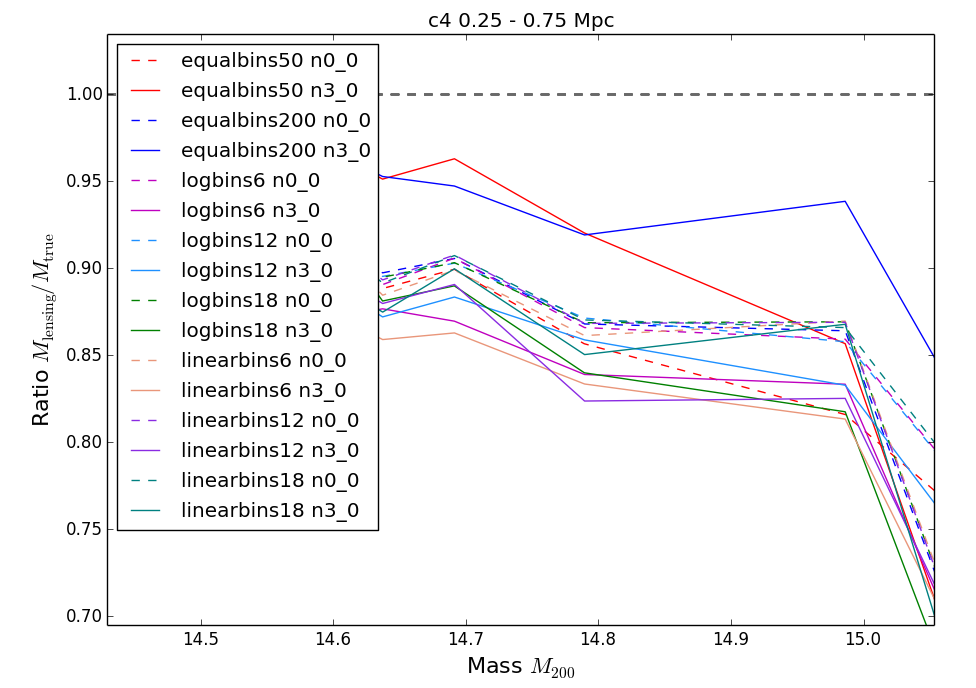
\includegraphics[width=0.45\textwidth]{figures/density_binning_core}
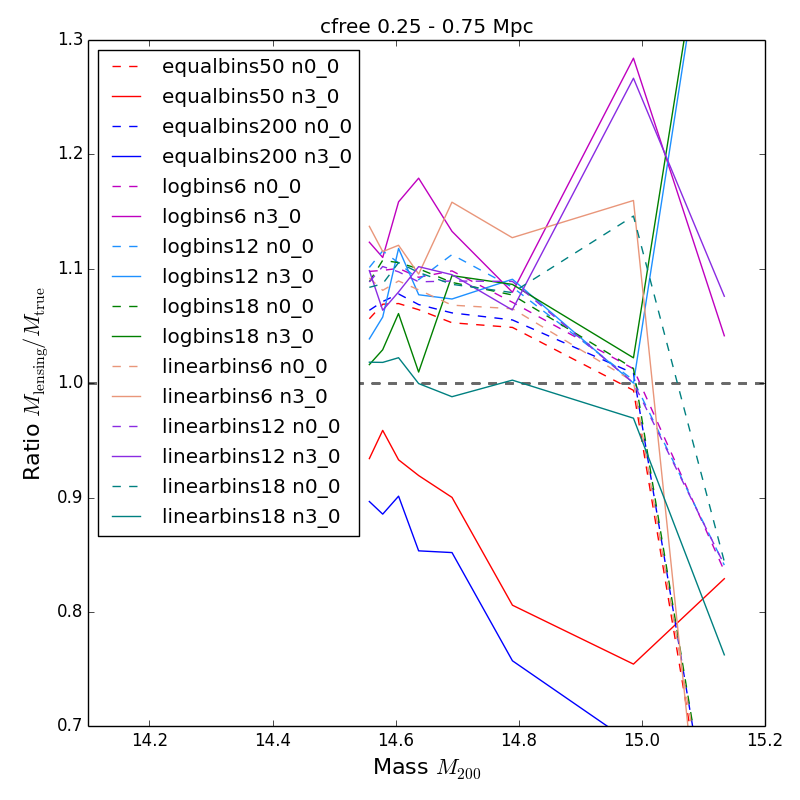
\includegraphics[width=0.45\textwidth]{figures/density_binning_core_cfree}\\
\caption{Comparison of bias at different densities and with different binning styles. For fits at high radius, binning style matters less than density. For the core, binning does matter, but at low densities, everything is very sensitive.}
\label{fig:density_binning_bias}
\end{figure}


Binning appears to have no effect on the scatter. Apparently these densities also have no effect on the scatter. 7 galaxies / arcmin must then still be high enough that intrinsic, correlated, and LoS structure is still the dominant noise source, at least for noise free shears.



%%%%%%%%%%%%%%%%%%%%%%%%%%%%%%%%%%%%%%%%%%%%%%%%%%%%%%%%%%%%%%
%%%%%%%%%%%%%%%%%%%%%%%%%%%%


\subsection{Next Steps}

I'd like to create perfect NFW halos, increase noise slowly, and inspect the posterior. That is probably the most clean way to investigate the effects of noise bias. However, what I'm concerned about is that the noise due to LSS \& substructure is not the same as shape noise, where noise is actually correlated between bins. I could imagine that correlated noise could induce difference effects. It would also be nice to model the amount of this correlated noise, so that I could include it in fits. 

%%%%%%%%%%%%%%%%%%%%%%%%%%%%%%%%%%%%%%%%%%%%%%%%%%%%%%%%%%%%%%%%%%%%%%%%%%%%%%%%%%%%%%%%%%%%%%%%%%%%%%%%%%%%%%%%%%%%%%%%%%%%%%%%%%%%%%%%%%%%%%%%%%%%%%%%%%%%%%%%%%%%%%%%%%%%%%%%%%%%%%%%%%%%%%%%%%%%%%%%%%%%
%%%%%%%%%%%%%%%%%%%%%%%%%%%%%%%%%%%%%%%%%%%%%%%%%%%%%%%%%%%%%%%%%%%%%%%%%%%%%%%%%%%%%%%%%%%%%%%%%%%%%%%%%%%%%%%%%%%%%%%%%%%%%%%%%%%%%%%%%%%%%%%%%%%%%%%%%%%%%%%%%%%%%%%%%%%%%%%%%%%%%%%%%%%%%%%%%%%%%%%%%%%%
%%%%%%%%%%%%%%%%%%%%%%%%%%%%%%%%%%%%%%%%%%%%%%%%%%%%%%%%%%%%%%%%%%%%%%%%%%%%%%%%%%%%%%%%%%%%%%%%%%%%%%%%%%%%%%%%%%%%%%%%%%%%%%%%%%%%%%%%%%%%%%%%%%%%%%%%%%%%%%%%%%%%%%%%%%%%%%%%%%%%%%%%%%%%%%%%%%%%%%%%%%%%
\clearpage \newpage

\section{What is the best configuration for the HST Program?}
\label{sec:hstproposal}


\subsection{Motivation}
There are a few different ways we could configure an HST program to observe high-redshift galaxy clusters. We can either take a single-pointing strategy, or some sort of mosaic. There are of course time limitions, and mosaicing will usually mean shallower exposures, with higher shape noise and lower galaxy density. The most effective strategy could also be redshift dependent, as the effective beta and sampling densities change.

\subsection{Setup}
I've used the MXXL to examine this question, by employing different instrument masks. I've introduced a few modifications so that I can approximate what happens when galaxy clusters are at different redshifts. This includes different source densities, different physical distances accepted into the analysis, and different effective betas. Modifications include a new reader class, readMXXL\_HSTBeta.py. 

I've used Tim's estimates of Beta, source density, and shape noise from the CANDELS fields. 

From Tim, on 19 Feb. (Note, I clarified that Beta here is $D_{ls}/D_s$, not normalized to $D_inf$.:
\begin{quotation}
Hi Doug,

here are my CANDELS estimates for our new HST program with source density, betas and shape noise:


After color cut ($V-i<0.4$ or $V-z<0.45$) and S/N cuts (Flux $S/N>10$):

Source density: (for V-i cut only so far) 

Single pointings: Ngal= 21/arcmin$^2$ ($24<V<26.5$) to $r=110"$, probably for $z>1$ clusters
[3-pt] Mosaics:          Ngal= 16/arcmin$^2$   ($24<V<26$)   to $r=160"$

Shape noise:
0.40 for both components together

Beta:
zl      beta
0.65  0.43  
0.70  0.40  
0.75  0.38   
0.80  0.36       
0.85  0.34   
0.90  0.32   
0.95  0.30   
1.00  0.28
1.05  0.26
1.10  0.24
1.15  0.23
1.20  0.21 
1.25  0.195
1.30  0.18

This is a bit pessimistic given that it uses uniform and not optimal weight, but this can be seen as margin.

Cheers, Tim
\end{quotation}

I've set up my code to ``move'' clusters to redshifts 0.7, 0.8, 0.9, 1.0, and 1.1. I've also tested single pointings, 3-pt mosiacs, and 4-pt mosaics based on the existing program. I've assumed the source density for the 4-pointing mosaics to be ~21 galaxies per square arcminute.


%%%%%%%%%%%%%%%%%%%%%%%%%%%%%%%%%%%%%%%%%%%%%%%%%%%%%%%%%%%%%%%%%%%%%%%%%%%%%%%%%%%%%%%%%%%%%%%%%%%%%%%%%%%%%%%%%%%%%%%%%%%%%%%%%%%%%%%%%%%%%%%%%%%%%%%%%%%%%%%%%%%%%%%%%%%%%%%%%%%%%%%%%%%%%%%%%%%%%%%%%%%%
%%%%%%%%%%%%%%%%%%%%%%%%%%%%%%%%%%%%%%%%%%%%%%%%%%%%%%%%%%%%%%%%%%%%%%%%%%%%%%%%%%%%%%%%%%%%%%%%%%%%%%%%%%%%%%%%%%%%%%%%%%%%%%%%%%%%%%%%%%%%%%%%%%%%%%%%%%%%%%%%%%%%%%%%%%%%%%%%%%%%%%%%%%%%%%%%%%%%%%%%%%%%
%%%%%%%%%%%%%%%%%%%%%%%%%%%%%%%%%%%%%%%%%%%%%%%%%%%%%%%%%%%%%%%%%%%%%%%%%%%%%%%%%%%%%%%%%%%%%%%%%%%%%%%%%%%%%%%%%%%%%%%%%%%%%%%%%%%%%%%%%%%%%%%%%%%%%%%%%%%%%%%%%%%%%%%%%%%%%%%%%%%%%%%%%%%%%%%%%%%%%%%%%%%%
\clearpage \newpage


\section{How many pointings do I need with PISCO?}
\label{sec:piscoproposal}


PISCO is a simultaneous imaging system being built at Harvard. It captures griz at the same time, so that each filter is seeing the same colors. This should mean that the colors are more accurate. Problem is, they only put one chip in it, with a field of view of 6x8'. It's kind of hard to probe out to 3Mpc with such a small chip, especially at the redshifts of MACS clusters ($0.3 < z 0.7$).

I came up with 3 different ways I could mosaic. Using 3 pointings, I could probe out along one axis, kind of like -:-. The long axis is 22 arcminutes, but the short one is only 8 arcminutes. With four pointings, I could either form a square that was $14\times14$ arcminutes, with little stubs off two sides. Or, I could make a cross with a hole in the center. Figuring each pointing is offset from the center by 1.5 arcminute, I could probe 1.5 - 9.5 arcminutes.

I set up each of these scenerios, plus a simple circular aperture with diameter 30 arcminute for comparison. While I'm not sure that the absolute scatters recorded are right, I'd think that the relative performance should be right. Figure~\ref{fig:piscoscatter} shows the relative performance. I'm a little surprised the circular aperature does less well at lower masses, but basically the 4 pointing strategy seems to work fine. Three pointings asymptotes to a higher scatter level, which should be avoided.

\begin{figure}
\centering
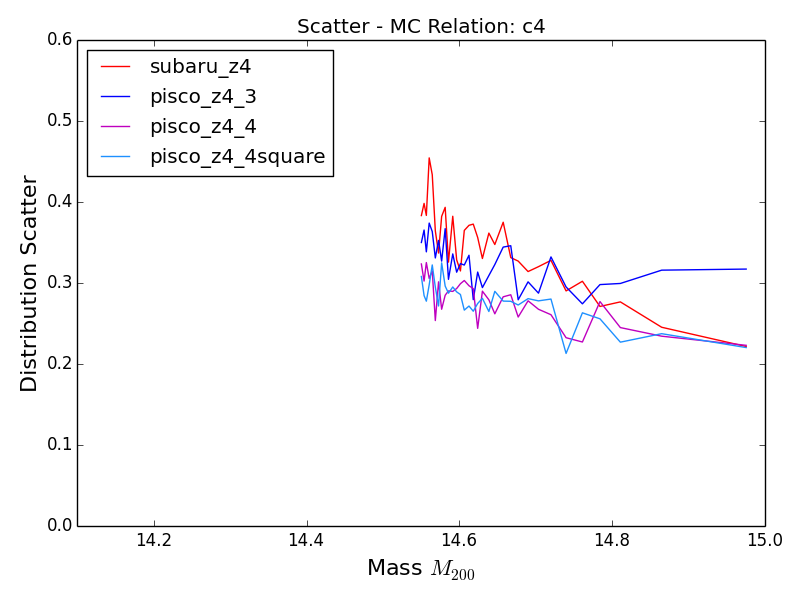
\includegraphics[width=0.65\textwidth]{figures/piscoproposal_scatter}
\caption{Expected Scatter (according to MXXL) as a function of cluster mass, for measuring M200. Four pointing solutions perform better than 3 pointings. Neither 4 pointing solution is a clear winner. Note that at lower masses, the most luxurious solution, the reference circle mask ``subaru'' actually has more scatter. That might be because it allows the profile to be measured all the way to 3Mpc. Could be a useful insight. }
\label{fig:piscoscatter}

\end{figure}




%%%%%%%%%%%%%%%%%%%%%%%%%%%%%%%%%%%%%%%%%%%%%%%%%%%%%%%%%%%%%%%%%%%%%%%%%%%%%%%%%%%%%%%%%%%%%%%%%%%%%%%%%%%%%%%%%%%%%%%%%%%%%%%%%%%%%%%%%%%%%%%%%%%%%%%%%%%%%%%%%%%%%%%%%%%%%%%%%%%%%%%%%%%%%%%%%%%%%%%%%%%%
%%%%%%%%%%%%%%%%%%%%%%%%%%%%%%%%%%%%%%%%%%%%%%%%%%%%%%%%%%%%%%%%%%%%%%%%%%%%%%%%%%%%%%%%%%%%%%%%%%%%%%%%%%%%%%%%%%%%%%%%%%%%%%%%%%%%%%%%%%%%%%%%%%%%%%%%%%%%%%%%%%%%%%%%%%%%%%%%%%%%%%%%%%%%%%%%%%%%%%%%%%%%
%%%%%%%%%%%%%%%%%%%%%%%%%%%%%%%%%%%%%%%%%%%%%%%%%%%%%%%%%%%%%%%%%%%%%%%%%%%%%%%%%%%%%%%%%%%%%%%%%%%%%%%%%%%%%%%%%%%%%%%%%%%%%%%%%%%%%%%%%%%%%%%%%%%%%%%%%%%%%%%%%%%%%%%%%%%%%%%%%%%%%%%%%%%%%%%%%%%%%%%%%%%%
\clearpage \newpage

\section{What is the best mass to measure?}

The above work was done looking at M200. However, as it currently stands, we are calibrating masses closer to M500. There is also an open question as to what mass is the least sensitive to m-c assumptions, or put another way, what is the mass that lensing measures the best?

To start, I'd like to remake the above plots with M500 instead of M200. However:

\begin{itemize}
\item The BCC M500 values appear to be larger than the M200 values
\item The MXXL M500 values that I have are for the z=0 slice, not the z=1 slice.
\end{itemize}

I've contacted Aaron about the MXXL problem, but I am holding off contacing Matt about the BCC issue until I am ready to show him some preliminary results.



%%%%%%%%%%%%%%%%%%%%%%%%%%%%%%%%%%%%%%%%%%%%%%%%%%%%%%%%%%%%%%%%%%%%%%%%%%%%%%%%%%%%%%%%%%%%%%%%%%%%%%%%%%%%%%%%%%%%%%%%%%%%%%%%%%%%%%%%%%%%%%%%%%%%%%%%%%%%%%%%%%%%%%%%%%%%%%%%%%%%%%%%%%%%%%%%%%%%%%%%%%%%
%%%%%%%%%%%%%%%%%%%%%%%%%%%%%%%%%%%%%%%%%%%%%%%%%%%%%%%%%%%%%%%%%%%%%%%%%%%%%%%%%%%%%%%%%%%%%%%%%%%%%%%%%%%%%%%%%%%%%%%%%%%%%%%%%%%%%%%%%%%%%%%%%%%%%%%%%%%%%%%%%%%%%%%%%%%%%%%%%%%%%%%%%%%%%%%%%%%%%%%%%%%%
%%%%%%%%%%%%%%%%%%%%%%%%%%%%%%%%%%%%%%%%%%%%%%%%%%%%%%%%%%%%%%%%%%%%%%%%%%%%%%%%%%%%%%%%%%%%%%%%%%%%%%%%%%%%%%%%%%%%%%%%%%%%%%%%%%%%%%%%%%%%%%%%%%%%%%%%%%%%%%%%%%%%%%%%%%%%%%%%%%%%%%%%%%%%%%%%%%%%%%%%%%%%
\clearpage \newpage

%%%%%%%%%%%%%%%%%%%%%%%%%%%%%%%%%%%%%%%%%%%%%%%%%%%%%%%%%%%%%%%%%%%%%%%%%%%%%%%%%%%%%%

\section{Understanding Maximum Likelihood Fits and Bootstrapping}

There is a lot of confusion about how to interpret maximum likelihood fits, bootstraping, and probability distributions.
I've added to the confusion.
So this is my attempt to straighten it out.

Let's start with Bayes Theorem.

\begin{equation}
P(\alpha|\vec y) \propto P(\vec y|\alpha)P(\alpha)
\end{equation}

Simple enough. When we do maximum likelihood, we ignore the prior.
Mathematically, that means $P(\alpha) = \mathrm{constant}$.

But what if we are not interested in $\alpha$, but instead $\beta = f(\alpha)$?
Bayes Rule give the same thing:

\begin{equation}
P(\beta|\vec y) \propto P(\vec y|\beta)P(\beta)
\end{equation}

Looking for the MLE is again equivalent to $P(\beta) = \mathrm{constant}$.
Since we are still looking at the same probability distribution, $\hat \beta$ that maximizes $P(\beta|\vec y)$ where $P(\beta) = \mathrm{constant}$, we have $\hat\beta = f(\hat\alpha)$ for $\alpha$ that maximized $P(\vec y|\alpha)$. 

But here's the paradax.
Imagine that we've mapped out $P(\alpha|\vec y) \ propto P(\vec y|\alpha)$, with $P(\alpha) = \mathrm{constant}$.
We can calculate $P(\beta|\vec y)$ from that distribution.

\begin{equation}
P(\beta|\vec y) = P(\alpha|\vec y)\frac{d\alpha}{d\beta}
\end{equation}

If $\beta = f(\alpha)$ is not linear, then $\frac{d\alpha}{d\beta} = f(\beta)$.
Substituting then, we have:

\begin{equation}
P(\beta|\vec y) = P(\alpha|\vec y)f(\beta) = P(\vec y|\alpha)f(\beta) = P(\vec y|\beta)P(\beta)
\end{equation}

This implies that in this case, we have $P(\beta) = \frac{d\alpha}{d\beta} = f(\beta)$.
That means this second $P(\beta|\vec y)$ is not identical to before, when we assumed $P(\beta) = \mathrm{constant}$.
Therefore, the MAP for $\beta$ is not $\hat \beta$.

Now, how do we interpret bootstrapping the MLE?
We obtain a bunch of samples of the MLE of $P(\vec y|\beta) = P(\vec y|\alpha)$ via bootstrapping.
What probability distribution to they correspond to?




%%%%%%%%%%%%%%%%%%%%%%%%%%%%%%%%%%%%%%%%%%%%%%%%%%%%%%%%%%%%%%%%%%%%%%%%%%%%%%%%%%%%%%%%%

\section{Immediate needs for SPT: Megacam-19 and HST-14}
\label{sec:spt_immediateneeds}

I need to get an answer for Tim and Joerg by the end of November of this month. The problem is still to figure out what exactly do they need from the simulations? How complicated do the predictions need to be?

What makes this hard to answer is that I don't think a constant offset number is going to be sufficient. The masses will be immediately plugged in to a scaling relation code, which will need the detailed relationship between true mass and lensing signal. The prior that will be assumed for the true mass is also going to change.

I think the minimum starting point has got to be measuring $P(g | m_{\mathrm{lens}})$. From that distribution, I can compute any needed summary info (without rerunning the pipeline), and I can apply any prior that I need. The domain for $m_{\mathrm{lens}|}$ has to be as unrestricted as possible, as the possible interpretations and priors will change, ie so that I can test allowing for negative mass, or different mass priors, etc.

That means I should get the mcmc sampling code running. Then I need to adjust the prior and make it improper. From there, I can run on all the simulations that I have, and then look at the posteriors and construct a model that describes all the data. Once I have the sampling from the likelihood, everything else should simply just be a reweighting of those chains.


Looking at the state of nfwfit.py, it looks like an MCMC sampling is already set up. However, the mass prior is restricted to be within a finite range. On the plus side, the concentration is independently sampled from the mass, so I should be able to immediate mimic a free concentration fit, and not worry about what the concentration should be for a negative mass.

The bigger problem with negative mass are the conversion functions between mass and scale radius. Let's inspect the posteriors with the standard $10^{[13,16]}$ prior, and see if any of the clusters get close to hitting the prior boundaries. That will tell us a lot right there.

What do I need to run? MCMC, log prior, cfree, 20k samples, fit ranges, noise \& density levels.

Then, miscentering with the same...


------


If I want to use the MCMC samples that I'm producing now for the current sample, I will need a way to summarize the information. I need to understand how I'm supposed to reqeight the samples so that I can recover a maximum likelihood  search.

Also, I need to understand what exactly do I need for Tim's and Joerg's papers. 

For Tim:
  - His paper is just going to be masses. So having some sort of average correction, or a mass dependent correction should be OK.

For Joerg:
  - His paper is feeding right into a scaling relations code. That code has $P(M_{lens} | M_{true})$ in it. 


Can I not just use what I already have?
  - I need to calculate M500 masses, so that is one thing that is different.
  - I need to make sure that their fits are run like my fits.
  - I need to understand how much of a noise dependence there is.

I have this old plot floating around from when I previously looked at noise dependence.
The results in that plot look rather scary, where there seems to be a big dependence on the prior.
In this case, it was simply a bounds prior.
Can I repeat that?




Looking at perfect NFW halos, and then plotting mfit / mtrue vs mtrue. The noise gets larger at lower masses, as to be expected, as noise is constant and signal is decreasing.
What is interesting is that the bias is more negative as we go to lower masses. 
This seems to be driven by a population of points that are hitting the prior boundary.

When I expand the boundary, to allow for masses to float down to 1e10, and higher, then down to a true mass of 2e14 I see that the bias is even lower. But at the lowest masses (< 2 e14), then I see that the bias switches directions and rises drastically.
This is despite a large population on thge lower boundary wall, and is instead a population that is scattering up.


I've now modified the code to fit a negative mass, by always taking the absolute value of the mass, and if negative, manually inserting a negative sign in front of the shear. In this case, and with a wide prior, the bias pretty much goes away!

So how do we best describe the noise?
If I plot the recovered distribution on a mass vs mass plot, I see an approximately equal amount of scatter. Though at the higher masses the scatter has a wider sigma than at lower masses!
This is best seen with a delta (not ratio) vs mass plot.


Just did a quick gaussian error propagation for M200 masses. $\sigma_M^2 = (\frac{dM}{dg})^2\sigma_g^2$. If we assume that we are just fitting the amplitude and not the shape, then $\frac{dr_s}{dg} = \mathrm{constant}$ and $\frac{dM}{dr_s} \propto r_s^2$, at least for $c=4$ models. Since there's a fixed noise in the shear profile, we expect the error to increase for higher masses, but the relative error will decrease!

But fine, this is all due to the noise in the shear profile, and not intrinsic noise. That should be captured from the uncertainties in the shear profile. But it also testifies to the fact that there is an intermediate stage object that COULD be negative in the analysis. 


Just checked what $\frac{dg}{dr_s}$ looks like. It is not a linear function of $r_s$. So there is no natural way to run this fit that is linear. So why is using no explicit prior an unbiased way to fit the masses?

Pumped up the errors in the shear profile to g $\pm1$, and I'm still not seeing any sign of nonlinearlity in the maxlike solution. Why not!? 
How does this change if I also fit for the concentration?

If you look at the quantity $\frac{d\gamma}{dr_s} = Kg(x)(1 - \frac{d\ln g}{d\ln x})$. So that would imply that the derivative 

Maybe it is roughly linear because I'm using the outer fit range. What happens if I use a more full radial range?


So I've now looked at the scatter and bias for a range of noise levels using a $c=4$ fit and using the innermost fit range, where I would expect nonlinear effects to be the highest. It still requires extremeley high noise levels to see any sort of biasing, and even then it seems to only kick in at the highest masses. So that would suggest that the extra contributions to the likelihood should be low.

One diagnostic of how bad things should be should be looking at the 2nd and 3rd derivates of the log posterior. If the ratio of the 3rd order Taylor expansion to the 2nd order taylor expansion along the 1-sigma boundary is large, I would expect to see noise bias issues.


I've now run noise bias tests for c constant and c free. With c constant, there just is not much of any noise bias to see, reflecting how the fit is nearly linear. However, with c free, the MLE estimate for mass is seriously biased upwards. Note that for cfree, it looks like the code adopts the Duffy M-C relation to generate the halos. The bias is proportionally much larger for light halos than massive halos. That supports the noise bias calculations from the last few days.

If we go back to the case where we limit the fit, then the will clearly be biases. The MLE will be pushed against the boundaries for some clusters, and when it is averaged, there will be a problem.


The reality of the situation, however, is that we will not use the MLE estimates. Or, if the posteriors are Gaussian when allowing for negative ``mass'', we could use that parameterization, with negative means.

The relevant question: How does handling the probability distribtions properly work? Sub-parts: In the c-free case, what does the probability distro for mass look like, after marginalizing out concentration? Is it Gaussian, is that MLE biased?

Even for low noise, the low mass case is not linear in either log or linear mass spacing. So if we want to fit for concentration, then we cannot use a Gaussian approximation. Problems are only worse at high noise.

Next question: How much noiser are the fits when we have cfree over c fixed? How many clusters do we need to beat down the extra noise to be below the systematic uncertainty of the m-c relations?

I started looking at this question. For fits to high radii, freeing the concentration does not seem to make much of a difference, probably because the concentration doesn't have a big effect. I need to rigorously quantify this, and check how things change as I go in to lower radii.

I also want to verify that the $P(M_{lens})$ that I produce from the marginalization process are accurate. The first way that comes to mind is to take all clusters with the same true mass and add their logprobs. I'm running that now, but that might not be definitive. The input to the test does not match the prior, and therefore I would not expect the test to return something sensible. I probably need to set up a CDF test.

Indeed, it appears that the multiplied probability is biased high by about 1e14. 

This is kind of strange. I ran a test with a prior. I generated masses uniform-log 14-16. I then measured the posterior for that range as well (hard prior boundaries). The CDF test shows a bias, towards underestimating the masses. Most of the problems are at the end points. 

Well, maybe this isn't a surprise. I fit for the concentration with a flat prior, but the clusters were all c=4. That could distort things. Let me check that.


\subsection{Fitting for bias \& Importance Sampling}
\label{sec:bias_framework}

Here are my notes from writing up how I'm planning to use the likelihood fits. Math as best as I can make it.

Definition of symbols: $\vec\alpha$ describes how I measure the bias and intrinsic scatter in weak lensing masses. $\vec\beta$ describe the true, 3D mass concentration relation. $M_t$ is the true mass, $M_l$ is the weak lensing mass, $c_l$ is the weak lensing ``effective'' concentration, ie, what weak lensing sees on the sky. $g$ is the shear profile.

I want to infer $P(\vec\alpha|M_t, c_t, g)$, ie what is the bias and scatter in lensing masses, given the true 3D parameters and the observed shear profile. The mass-concentration relation is marginalized over.

Rearranging terms by repeated aplication of Bayes Rule/Conditional Probability, I get:

\begin{equation}
P(\vec\alpha|M_t, c_t, g) = P(g|M_t,c_t,\vec\alpha)P(\vec\alpha)\frac{P(M_t,c_t)}{P(M_t,c_t,g)}
\end{equation}

Since $M_t$, $c_t$, and g are given, we can take the prior probabilies $P(g)$, $P(M_t)$, and $P(c_t)$ as constants that we can ignore. To connect the true quantitites with the shear profile, we introduce and marginalize out the inferred lensing quantities $M_l$ and $c_l$.

\begin{equation}
P(g|M_t,c_t,\vec\alpha)P(\vec\alpha) = P(\vec\alpha)\int_{\forall M_l, c_l} P(g|M_l,c_l)P(M_l,c_l|M_t,c_t,\vec\alpha)dM_ldc_l
\label{eq:marginalization}
\end{equation}

This is written for one cluster. I will suppress the generalization for many clusters. Ahead of time, we have already MCMC sampled the likelihood for one cluster. 

\begin{equation}
P(M_l,c_l|g)^{\prime} = P(g|M_l,c_l)P(M_l,c_l)^{\prime}
\end{equation}

It is important to notice that the prior distriubtion used to sample the likelihood for an individual cluster can generally have \emph{no relation} to the prior probabilities in the problem that we actually want to solve. We want to evaluate the function from equation~\ref{eq:marginalization} with a Monte Carlo method. Specifically, we want to use the likelihood chains that we have already drawn for the individual cluster.

\begin{align}
\int_{\forall M_l, c_l} P(g|M_l,c_l)P(M_l,c_l|M_t,c_t,\vec\alpha)dM_ldc_l \\
  = \int_{\forall M_l, c_l} \frac{P(g|M_l,c_l)P(M_l,c_l|M_t,c_t,\vec\alpha)}{P(M_l,c_l|g)^{\prime}}P(M_l,c_l|g)^{\prime}dM_ldc_l \\
  = \frac{1}{n}\sum\limits_{M_l^{\prime},c_l^{\prime}}\frac{P(g|M_l,c_l)P(M_l,c_l|M_t,c_t,\vec\alpha)}{P(M_l,c_l|g)^{\prime}} \\
  = \frac{1}{n}\sum\limits_{M_l^{\prime},c_l^{\prime}}\frac{P(g|M_l,c_l)P(M_l,c_l|M_t,c_t,\vec\alpha)}{P(g|M_l,c_l)P(M_l,c_l)^{\prime}} \\
  = \frac{1}{n}\sum\limits_{M_l^{\prime},c_l^{\prime}}\frac{P(M_l,c_l|M_t,c_t,\vec\alpha)}{P(M_l,c_l)^{\prime}} \\
\end{align}

In the above equations, we are turning the integration over all $M_l$ and $c_l$ into a summation over samples via Monte Carlo integration. However, we are pulling from the primed distribution, so we need to multiply and divide by it first. That's the importance sampling bit: each sample is weighted by the ratio of the probability distributoon we care about over the probability distribution we sampled from. However, the shear profile likelihood is evaluated in each, and therefore cancels. The remaining weight is simply the prior that we assumed when we sampled $M_l$ and $c_l$ for each cluster. 

Here it is important to pay attention to which variable we are actually integrating over. Are we integrating over $M_l$ and $c_l$ or $\log M_l$ and $\log c_l$. The weight can be ignored if the variable we are integrating in had a uniform prior when we were sampling each individual prior.

%%%%%%%%%%%

I have finally run the model on some fake data, and I don't like what I'm seeing. There appears to be a bias in the ratio, and it gets more negative at higher masses. I do not know why.

The inferred mass scatter is also wrong. For the lowest mass bins, the scatter is inferred to be too large.

Again with concentration, there is a systematic trend where low masses overestimate and high masses underestimate.

Concentration scatter is across the board underestimated. 

And probably because of all that (or causing it?) the mc covar has the wrong sign.


%%%%%%%%%%%%%%%%%%%%%%%%%%%%%%%%%%%%%%%%%%%%%%%%%%%%%%%%%%%%%%%%%%%%%%%%%%%%%%%%%%%%%%%%%%%%%%%%%%%%%%%%%%%%%%%%%%%%%%%%%%%%%%%%%%%%%%%%%%%%%%%%%%%%%%%%%%%%%%%%%%%%%%%%%%%%%%%%%%%%%%%%%%%%%%%%%%%%%%%%%%%%
%%%%%%%%%%%%%%%%%%%%%%%%%%%%%%%%%%%%%%%%%%%%%%%%%%%%%%%%%%%%%%%%%%%%%%%%%%%%%%%%%%%%%%%%%%%%%%%%%%%%%%%%%%%%%%%%%%%%%%%%%%%%%%%%%%%%%%%%%%%%%%%%%%%%%%%%%%%%%%%%%%%%%%%%%%%%%%%%%%%%%%%%%%%%%%%%%%%%%%%%%%%%
%%%%%%%%%%%%%%%%%%%%%%%%%%%%%%%%%%%%%%%%%%%%%%%%%%%%%%%%%%%%%%%%%%%%%%%%%%%%%%%%%%%%%%%%%%%%%%%%%%%%%%%%%%%%%%%%%%%%%%%%%%%%%%%%%%%%%%%%%%%%%%%%%%%%%%%%%%%%%%%%%%%%%%%%%%%%%%%%%%%%%%%%%%%%%%%%%%%%%%%%%%%%
\clearpage \newpage


\section{Miscentering}

We know that the SZ centers are rather noisy. How much of an effect does that have on the inferred bias?

I have a file from hydro sims provided by Jiayi. It has clusters of different masses and redshifts with simulated SZ data. 

There are a number of variables that could matter. Mass, redshift, SN, and coresize. There is a correlation between delta r and coresize.


%%%%%%%%%%%%%%%%%%%%%%%%%%%%%%%%%%%%%%%%%%%%%%%%%%%%%%%%%%%%%%%%%%%%%%%%%%%%%%%%%%%%%%%%%%%%%%%%%%%%%%%%%%%%%%%%%%%%%%%%%%%%%%%%%%%%%%%%%%%%%%%%%%%%%%%%%%%%%%%%%%%%%%%%%%%%%%%%%%%%%%%%%%%%%%%%%%%%%%%%%%%%
\clearpage \newpage


\section{Effects of Miscentering}

I have used simulations from Jiayi to characterize how the SZ center is offset from the DM center as a function of the SPT detection properties. The distribution of miscentering is primarily dependent on the core-size used to filter the maps for detection, with a secondary dependence on mass and/or significance.

[Insert figures that describe that distribution here].

I have set up to run on mxxlsnap41 and bk11snap141 to characterize the effect of miscentering on the mass bias at the HST and Megacam redshifts. For the initial run, I ran with three noise levels and three core sizes (plus one control). I'm restricting to using mass-concentration relations, since that makes the distributions gaussian, and is closer to what is being done by Joerg and Tim. These two snaps also have the advantage that I know the m500 values.


First question: What does the distribution shape look like between $m_{true}$ and $m_{meas}$?

Looking at the mxxl, the distribution for the bias is not lognormal. There is a tail to overestimated masses at a fixed true mass, and the median of the pull is negative.  Is that duplicated in bk11? Yes. And it can be seen in figure 3 of BK11.

Note that this tail to overestimated masses is not due to noise in the true mass estimates. Or, to put it another way, the true mass estimates would need to have larger errors than the measured mass estimates to have a tail to overestimated masses. Seems unlikely. I'll have to leave investigating these odd tail cases to later.

Some of the fit files, in particular mxxl c4 r5 n3\_2 and n4\_3 appear to have multiple fit failures with nans corrupting the file. Will need to investigate that.

At least for the 0.75 - 2.5 fit range and at low masses, the noise level does appear to make a difference! That is surprising given my tests on perfect NFW halos.  OK, looking back in notes.pdf, maybe it isn't so surprising at the lowest sampling level. I need to look at this in more detail to make sure I understand it.


I compared the observed offset distribution from Jiayi's sims to a simple analytic model that Brad proposed. That model is a .3 arcmin gaussian scatter with a 100kpc gaussian scatter. The first is due to noise effects in the SZ detection (as determined in comparison to X-ray obs) and the second is a physical offset between Planck SZ and BCG peaks, representing cluster intrinsic shapes. That model seems to describe the simulations reasonably well, at least where we actually have clusters.

\logfig{figures/offsetdistro_vs_analytic}{Comparison of simulation offset distributions to an analytic model of two convolvued gaussians. The blue line is from Jiayi's simulations. The green line is the miscentering distribution assuming a gaussian scatter with width sqrt(.3 arcmin ^ 2 + 100kpc@mean(clusterz)).}



%%%%%%%%%%%%%%%%%%%%%%%%%%%%%%%%%%%%%%%%%%%%%%%%%%%%%%%%%%%%%%%%%%%%%%%%%%%%%%%%%%%%%%%%%%%%%%%%%%%%%%%%%%%%%%%%%%%%%%%%%%%%%%%%%%%%%%%%%%%%%%%%%%%%%%%%%%%%%%%%%%%%%%%%%%%%%%%%%%%%%%%%%%%%%%%%%%%%%%%%%%%%
\clearpage \newpage

\section{Measuring Total Bias for HST Sample}

I'm trying to boil down the correction factor for HST, using all the elements.The first problem I'm having, however, is that I don't know how to describe the distribution coming from the simulations when there is noise.

It's clear from other plots that with no noise, the distribution is not log-normal. When we add noise, part of the distribution is coming from the noise already accounted for in the statistical errors. The rest I need to characterize.

One problem is that if you look at measured mass - true mass (the linear quantity), I would have expected to see a Gaussian distribution. That is because the fit should be almost linear, and in a linear fit the posterior is gaussian. 

One major problem may simply be the number of radial bins in the profile. For one cluster that I checked, the shear profile that I'm fitting to has one datapoint. This is due to the downsampling to match the density of points available. 

Note: This section was down on 19 Jan 2015, after I fixed the number density numbering issue.



The bias in m200 is flat with mass. The bias in m500 turns positive at low masses. Why??? 
This is probably a selection effect. We have all clusters down to a mass m200. However, for clusters of a particular mass m200, there will be a range of m500s, which will depend on the concentration of the halo. The halos that are selected are only those m500s where m200 meets our threshold, implying a selection on m500 and concentration.


I found the problem with the noise tests! As I reduced the number of samples in the catalog, the equal binning shear profile algorithm started throwing away bins. So that meant for the noisest sampling, my shear profile had only one point. That is why the noise apparent in M_lens / M_true was much higher than I expected. I switched to 12 bin linear binning, which is approximately what Tim is using for the paper. (Prior tests show that the exact number of bins shouldn't matter too much, but I suppose I could try to exactly match Tim's algorithm later). I'm about to check what those distributions look like.


Further update. I've run the noise tests. The initial results seem to suggest that there is a HUGE noise bias problem. Specifically, the bias can be up to a factor of 2x. I don't belive this. If this is true, this is a major. One hint that there is some other problem: The magnitude of the intrinsic scatter is not constant, or decreasing with increasing noise (as I would expect, since it is constant, and harder to detect). It is instead increasing with increasing noise. A quick flip through some of the fits, I worry that the fits are not converging to a proper value, that there is something that is stopping the fits prematurely. My next step is to check the chisq distribution for the fits, to see if it is reasonable. Another possibility is that there is a likelihood barrier at zero mass that might be messing up the fits. 

In checking the chisq tests, not every fit uses the same number of data points. This is because the profile drops radial bins with less than five galaxies. I'm a bit surprised that some profiles only have 6 datapoints (the lowest that I see). Looking at the histogram of cdf values, it is very clear that way too many fits have too high of a chisq. (OK, maybe this is not surprising, considering that there is intrinsic scatter that I'm trying to measure). 


From spot checking a few catalogs, it does not appear that the fitting algorithm is having a problem. The fits all seem to be working reasonably well. So that to me is suggesting that the lognorm model is not a good description of the data. That's the next to check. I might also need to rerun fits where I keep no shape noise, but decrease the density of points, to see how that alters the intrinsic noise distribution shape.

Conferred with Anja. She things its a binning issue. Two few galaxies per bin might mean that the bootstrap isn't fully capturing the uncertainty in each shear bin. I'll set up a run9 to test different binning strategies. I will also remove the ngal < 5 drop constraint.





%%%%%%%%%%%%%%%%%%%%%%%%%%%%%%%%%%%%%%%%%%%%%%%%%%%%%%%%%%%%%%%%%%%%%%%%%%%%%%%%%%%%%%%%%%%%%%%%%%%%%%%%%%%%%%%%%%%%%%%%%%%%%%%%%%%%%%%%%%%%%%%%%%%%%%%%%%%%%%%%%%%%%%%%%%%%%%%%%%%%%%%%%%%%%%%%%%%%%%%%%%%%
%%%%%%%%%%%%%%%%%%%%%%%%%%%%%%%%%%%%%%%%%%%%%%%%%%%%%%%%%%%%%%%%%%%%%%%%%%%%%%%%%%%%%%%%%%%%%%%%%%%%%%%%%%%%%%%%%%%%%%%%%%%%%%%%%%%%%%%%%%%%%%%%%%%%%%%%%%%%%%%%%%%%%%%%%%%%%%%%%%%%%%%%%%%%%%%%%%%%%%%%%%%%
%%%%%%%%%%%%%%%%%%%%%%%%%%%%%%%%%%%%%%%%%%%%%%%%%%%%%%%%%%%%%%%%%%%%%%%%%%%%%%%%%%%%%%%%%%%%%%%%%%%%%%%%%%%%%%%%%%%%%%%%%%%%%%%%%%%%%%%%%%%%%%%%%%%%%%%%%%%%%%%%%%%%%%%%%%%%%%%%%%%%%%%%%%%%%%%%%%%%%%%%%%%%
\clearpage \newpage

\section{Collaborators, Acknowledgements, Debts}

\subsection{Collaborators}

Stanford
\begin{itemize}
\item Steve Allen
\item Anja von der Linden
\item Pat Kelly
\item Adam Mantz
\item Glenn Morris
\end{itemize}

Bonn
\begin{itemize}
\item Tim Schrabback
\item Peter Schneider
\end{itemize}

SPT
\begin{itemize}
\item Brad Benson
\item Joerg Dietrich
\end{itemize}

MXXL Simulations
\begin{itemize}
\item Stefan Hilbert
\end{itemize}

BCC Simulations
\begin{itemize}
\item Risa Wechsler
\item Matt Becker
\item Michael Buscha
\end{itemize}

BK11 Simulations
\begin{itemize}
\item Matt Becker
\end{itemize}


%%%%%%%%%%%%%%%%%%%%%%%%%%%%

\bibliography{refs.bib}

%%%%%%%%%%%%%%%%%%%%%%%%%%%%%



\end{document}

